\documentclass[review,authoryear]{elsarticle}

\usepackage{graphicx}
\usepackage{pstricks}
\usepackage{multido}
\usepackage[utf8]{inputenc}

\usepackage{lineno}
\linenumbers

\newcommand{\eq}[2]{\begin{equation}\label{#2}#1\end{equation}}
\newcommand{\sign} {\mathrm{sign}}
\newcommand{\PARTIAL}[2] {\frac{\partial#1}{\partial#2}}
\newcommand{\D}[3] {\frac{d^{#3} #1}{d #2^{#3}}}
\newcommand{\I}[2] {\frac{\delta #1}{\delta #2}}
\newcommand{\PA}[1] {\left(#1\right)}
\newcommand{\C}[1] {\left[#1\right]}
\newcommand{\LL}[1] {\left\{#1\right\}}
\newcommand{\ABS}[1] {\left|#1\right|}
\newcommand{\MATRIX}[2] {\PA{\begin{array}{#1}#2\end{array}}}
\newcommand{\si}{\mathrm{if}}

\newcommand{\IR}{_{i+(1/2)}}
\newcommand{\IRR}{_{i+(3/2)}}
\newcommand{\IL}{_{i-(1/2)}}
\newcommand{\ILL}{_{i-(3/2)}}

\bibliographystyle{elsarticle-harv}

\begin{document}

\title
{
	SURCOS: a software tool to simulate irrigation and fertigation in isolated 
	furrows and furrow networks
}

\author[rvt1,rvt3]{J.~Burguete\corref{cor1}}
\ead{jburguete@eead.csic.es}

\author[rvt2]{A.~Lacasta}
\ead{alacasta@unizar.es}

\author[rvt2]{P.~García-Navarro}
\ead{pigar@unizar.es}

\cortext[cor1]{Corresponding author}
\address[rvt1]{Soil and Water, EEAD / CSIC.
P.O. Box 13034, 50080~Zaragoza, Spain.}
\address[rvt2]{Fluid Mechanics, LIFTEC, CSIC-Universidad de Zaragoza.
María de Luna 3, 50018~Zaragoza, Spain.}
\address[rvt3]{BIFI: Instituto de Biocomputación y Física de Sistemas Complejos,
Universidad de Zaragoza.
Mariano Esquillor, Edificio I+D, 50009~Zaragoza, Spain.}

\begin{keyword}
simulation software, infiltration, furrows, irrigation, fertigation
\end{keyword}

\begin{abstract}
A software tool useful for the numerical computation of surface irrigation and
fertigation in furrows and furrow networks was developed. The model solves the
complete one-dimensional St-Venant equations together with the transport
equation of a passive solute. The flow equations and the solute advection are
solved with a high resolution TVD explicit Eulerian scheme. The solute
dispersion is solved with a centered implicit Eulerian scheme to avoid further
restriction in the allowable time step. The computational speed of the model is
high in isolated furrows. In cases of large furrow networks over extended
irrigation times the model is slower but affordable computational speed is
achieved. The computational model has been designed to be robust, intuitive and
able to supply useful visual results. Both the executable and the source code,
as well as the examples presented can be downloaded, edited and distributed
under a BSD type license.
\end{abstract}

\maketitle

\section{Introduction}

Engineering studies of surface irrigation systems begin with an evaluation of
current performance based on field-measured data in order to determine the
applied amount of the irrigation water. The interest is in the distribution of
infiltrated water along the field in order to evaluate whether water contributed
to satisfy the irrigation requirement and how much was lost by deep percolation
and runoff. The ultimate objective is to identify recommendations that result in
acceptable levels of irrigation performance under the expected range of field
conditions.

In the last decades computer based models were developed to support this
analytical process. The most usual simulation engines, WinSRFR
\citep{Clemmens99} and SIRMOD \citep{Walker03}, can be configured to model
basins, borders, and furrows, all under the assumption of one-dimensional flow.
This means that all flow characteristics vary only with distance along the field
length and time, i.e. not across the field width. For borders and basins, the
models are applicable to situations where the side-fall is negligible in
comparison with the applied depth, infiltration and roughness are relatively
uniform across the field width, and inflow is distributed. With furrows,
simulations consider only a single furrow and, therefore, neighboring furrows
are assumed identical. Any variation in properties from furrow to furrow must be
modeled separately. Their simulation engines solve the one-dimensional unsteady
open-channel flow equations coupled with empirical/semi-empirical equations
describing infiltration and channel roughness. The governing equations represent
the physical principles of conservation of mass and momentum. Given the
relatively low velocities and Froude numbers that characterize
surface-irrigation flows, their simulation engines often solve truncated forms
of the momentum equation. The zero-inertia (force equilibrium) version assumes
only pressure gradients, friction, and gravitational forces acting on the flow. 
Examples of recent applications of these models can be
\cite{Bautista09a,Bautista09b} or \cite{EbrahimiamLiaghat11}.
Other irrigation models such as \cite{Mailapalli09} or \cite{Soroush13} have been reported but they don't offer an easy and user friendly software tool.

Water flow simulation in open channels and rivers has been a topic of interest
recently and many numerical advances can be found. They include the presence of
transcritical flow, bed slope changes, non-oscillatory high order calculations
\citep{JaviTVD}, unsteady boundary conditions \citep{JaviContorno}, solute
transport \citep{JaviTrans} and dominant friction terms
\citep{JaviFriccion,JaviFriccion2}. In order to extend those developments to
furrow irrigation simulation, specific models have been adapted to formulate
friction, solute dispersion, infiltration and junctions in furrows and furrow
networks \citep{JaviSurcos1,JaviSurcos2}.

The objective of the present work is the development of a software tool to
simulate the complete water flow dynamics and solute transport in furrows and
furrow networks with a basis on the exhaustive verification and validation
performed in \cite{JaviSurcos1,JaviSurcos2}. The software \emph{SURCOS} has been
designed to incorporate the cited modelling improvements in a user friendly,
reliable, robust and efficient tool.

First, the governing equations used are outlined in order to state the notation.
Second, the numerical scheme used in the simulation engine is detailed to enable
an easy reproduction of the model. Then, the main components of the software
interface are presented. Finally, some examples of use are included to
illustrate the performance.

The model and the examples presented in this work are distributed
\citep{Surcos,SurcosGit} as free software under a Berkeley Software Distribution
(BSD) type license with available and editable source code.

\section{Physical model}

\subsection{Shallow-water model}

The one-dimensional system formed by the cross sectional averaged liquid and
solute mass conservation, momentum balance in main stream direction,
infiltration and solute transport in prismatic open channels can be expressed in
conservative form as \citep{JaviSurcos1}:
\eq
{
	\PARTIAL{\vec{U}}{t}+\PARTIAL{\vec{F}}{l}=
	\vec{I}+\vec{S}^c+\PARTIAL{\vec{D}}{l},
}{EqCons}
where $\vec{U}$ is the vector of conserved variables, $t$ is the time, $\vec{F}$
the flux vector,  $l$ the longitudinal coordinate, $\vec{I}$ the infiltration
vector, $\vec{S}^c$ the source term vector, and $\vec{D}$ stands for solute
dispersion:
\[
	\vec{U}=\MATRIX{c}{A\\Q\\A\,s},\quad
	\vec{F}=\MATRIX{c}{Q\\g\,I_1+\frac{Q^2}{A}\\Q\,s},\quad
	\vec{S}^c=\MATRIX{c}{0\\g\,A\,\PA{S_0-S_f}\\0},
\]
\eq
{
	\vec{I}=\MATRIX{c}{-P\,I\\0\\-P\,I\,s},\quad
	\vec{D}=\MATRIX{c}{0\\0\\K_l\,A\PARTIAL{s}{l}},
}{EqVar}
with $A$ the wetted cross sectional area, $Q$ the discharge, $s$ the cross
sectional average solute concentration, $g$ the gravity acceleration, $S_0$ the
longitudinal bottom slope, $S_f$ the longitudinal friction slope, $K_l$ the
longitudinal solute dispersion coefficient, $I$ the infiltration rate, $P$ the
cross-sectional wetted perimeter and $I_1$ represents pressure forces.

The furrows are modeled as pervious prismatic channels of trapezoidal cross
section as represented in Figure~\ref{FigSurco}. In this case, the pressure
integral becomes \citep{JaviSurcos1}:
\eq{I_1=\frac{B_0\,h^2}{2}+\frac{Z\,h^3}{3},}{EqII}
The set of equations is completed with the laws for infiltrated volume of water
and solute \citep{JaviSurcos1}:
\eq{\PARTIAL{\alpha}{t}=P\,I,\quad\PARTIAL{\phi}{t}=P\,I\,s,}{EqMassInf}
with $\alpha$ the volume of water infiltrated per unit length of furrow and
$\phi$ the mass of solute infiltrated per unit length of the furrow.
\begin{figure}[ht]
\centering
\begin{picture}(340,110)
	\multiput(0,0)(170,0){2}
	{
		\put(0,90){\line(1,-1){50}}
		\put(50,40){\line(1,0){50}}
		\put(100,40){\line(1,1){50}}
		\put(150,90){\line(1,0){20}}
		\qbezier[10](0,90)(0,95)(0,100)
	}
	\put(0,95){\vector(1,0){170}}
	\put(170,95){\vector(-1,0){170}}
	\put(80,100){$W$}
	\qbezier[50](50,40)(50,65)(50,90)
	\qbezier[50](100,40)(100,65)(100,90)
	\put(20,70){\vector(1,0){30}}
	\put(50,70){\vector(-1,0){30}}
	\put(50,70){\vector(1,0){50}}
	\put(100,70){\vector(-1,0){50}}
	\put(100,70){\vector(1,0){30}}
	\put(130,70){\vector(-1,0){30}}
	\put(75,40){\vector(0,1){30}}
	\put(75,70){\vector(0,-1){30}}
	\put(25,75){$Z\,h$}
	\put(70,75){$B_0$}
	\put(105,75){$Z\,h$}
	\put(77,50){$h$}
	\put(10,10){\vector(1,0){20}}
	\put(10,10){\vector(0,1){20}}
	\put(0,30){$z$}
	\put(30,0){$y$}
	\put(75,10){\vector(0,1){30}}
	\put(77,20){$z_b$}
	\qbezier[70](100,40)(135,40)(170,40)
	\put(160,40){\vector(0,1){50}}
	\put(160,90){\vector(0,-1){50}}
	\put(162,60){$H$}
\end{picture}
\caption{Trapezoidal furrow geometry. $h$ is the water depth, $W$ the
	distance between furrows, $z_b$ the bottom level, $H$ the furrow depth,
	$B_0$ the base width and $Z$ the tangent of the angle between the furrow
	walls and the vertical direction.\label{FigSurco}}
\end{figure}

The Jacobian matrix of the flow can be expressed as \citep{JaviSurcos1}:
\eq
{
	\mathbf{J}=\PARTIAL{\vec{F}}{\vec{U}}=
	\MATRIX{ccc}{0&1&0\\c^2-u^2&2u&0\\-u\,s&s&u},
}{EqJac}
where $u=\frac{Q}{A}$ is the cross sectional average velocity,
$c=\sqrt{\frac{g\,A}{B}}$ is the velocity of the infinitesimal waves and
$B$ is the cross section top width.
This matrix can be made diagonal \citep{JaviSurcos1}:
\eq
{
	\mathbf{J}=\mathbf{P}\,\mathbf{\Lambda}\,\mathbf{P}^{-1},\quad
	\mathbf{P}=\MATRIX{ccc}{1&1&0\\\lambda^1&\lambda^2&0\\s&s&1},\quad
	\mathbf{\Lambda}=\MATRIX{ccc}{\lambda^1&0&0\\0&\lambda^2&0\\0&0&\lambda^3},
}{EqPPL}
with $\mathbf{\Lambda}$ the eigenvalues diagonal matrix, $\mathbf{P}$ the
diagonalizer matrix and $\lambda^k$ the Jacobian eigenvalues corresponding to
the propagation characteristic celerities:
\eq{\lambda^1=u+c,\quad\lambda^2=u-c,\quad\lambda^3=u.}{EqLambda}

\subsection{Furrow infiltration model}

The infiltration rate is calculated using the Kostiakov-Lewis model modified by
\cite{JaviSurcos1} in furrows:
\eq{I=I_c+K\,a\,\PA{\frac{\alpha}{K\,W}}^\frac{a-1}{a},}
{EqKostiakovLewisSurcosi}
where $K$ is the Kostiakov constant and $a$ is the Kostiakov exponent, both
empirical parameters depend on soil type, soil water and compaction, and $I_c$
is the saturated infiltration long-term rate \citep{WalkerSkogerboe87}.

\subsection{Friction model}

The friction slope can be modeled by means of the Gauckler-Manning law
\citep{Gauckler,Manning} that, for a furrow of trapezoidal cross section is
\citep{JaviSurcos1}:
\eq
{
	S_f=\frac{n^2\,Q\,|Q|\PA{B_0+2\,h\,\sqrt{1+Z^2}}^{4/3}}
	{\PA{B_0\,h+Z\,h^2}^{10/3}}.
}{EqManning}

The model can calculate the friction with the model proposed in
\cite{JaviFriccion,JaviFriccion2}, that in furrows with trapezoidal cross
section is \citep{JaviSurcos1}:
\eq
{
	S_f=\frac{\epsilon\,(b+1)^2\,d^{2\,b}\,|Q|\,Q}
	{g\,\LL{B_0\,\PA{h^{b+\frac32}-\sqrt{h}\,d^{1+b}}+
	2\,Z\,\C{\frac{h^{b+\frac52}-d^{b+\frac52}}{b+\frac52}-
	\frac{2}{3}d^{1+b}\,\PA{h^\frac32-d^\frac32}}}^2},
}{EqSf}
where $b$ is a fitting exponent of the vertical profile of flow velocity, $d$ is
a characteristic length of the bed roughness irregularities, $\epsilon$ is a
dimensionless parameter of aerodynamical resistance depending only, in turbulent
flows, on the roughness shape. In furrows, $b=0.27$ is used based in rivers
measurements \citep{JaviFriccion}. This friction law is only valid for $h>d$. If
$h<d$ a zero velocity condition ($Q=0$) is imposed.

\subsection{Solute dispersion model}

The diffusion coefficient contains all the information related to molecular or
viscous diffusion, turbulent diffusion and dispersion derived from the averaging
process. A model suggested in \cite{Rutherford94} will be used for practical
applications:
\eq{K_l=10\,\sqrt{g\,P\,A\,\ABS{S_f}}.}{EqRutherford}

\section{Numerical model}

\subsection{Mesh}

\begin{figure}[ht]
	\centering
	\begin{tabular}{cc}
		(a)&(b)\\
		\begin{picture}(145,145)
			\put(0,85){$\PA{x_1,\,y_1}$}
			\put(110,60){$\PA{x_2,\,y_2}$}
			\put(20,75){\line(5,-1){110}}
			\put(35,75){Distribution furrow}
		\end{picture}&
		\begin{picture}(175,145)
			\put(0,135){$\PA{x_1,\,y_1}$}
			\put(110,110){$\PA{x_2,\,y_2}$}
			\put(20,125){\line(5,-1){110}}
			\put(35,125){Distribution furrow}
			\multiput(20,125)(11,-2.2){11}{\line(1,-6){15}}
			\put(30,85){Irrigation furrows}
			\put(30,70){1}
			\put(41,67.8){2}
			\put(85,59){$i$}
			\put(140,48){$N_{furrows}$}
			\put(10,20){$\PA{x_3,\,y_3}$}
			\put(35,35){\line(5,-1){110}}
			\put(130,0){$\PA{x_4,\,y_4}$}
			\put(45,10){Recirculation furrow}
		\end{picture}
	\end{tabular}
	\caption{Possible geometry configurations in \emph{SURCOS}: (a) isolated
		furrow ($N_{furrows}=0$), where only the distribution furrow is
		simulated, (b) furrow irrigation network ($N_{furrows}>0$). The
		recirculation furrow is optional.\label{FigGeometry}}
\end{figure}

In every furrow, the discrete mesh longitudinal coordinates are defined as:
\eq{l_i=\frac{i-1}{N-1}\,L,}{EqMeshPositions}
with $l_i$ the longitudinal coordinate, $N$ the number of cells discretizing the
furrow and $L$ the furrow length. The size of every cell $\delta l_i$ and the
distance between cells $\delta l\IR$ is defined as:
\[
	\delta l\IR=l_{i+1}-l_i=\frac{L}{N-1},
\]
\eq
{
	\delta l_i=\frac{L}{N-1},\;(i<N\;\mathrm{and}\;i>1),\quad
	\delta l_1=\delta l_N=\frac12\,\frac{L}{N-1}.
}{EqMeshSize}

The model can only be used for furrows of uniform slope. The
grid cells bed level is computed by interpolation from the furrows end points.

\subsection{Sub-steps}

The numerical scheme used in this paper is based on a seven sub-steps algorithm
very similar to the proposed in \cite{JaviSurcos1}:
\begin{enumerate}
\item In the first sub-step, the flow equations and the advective part of the
transport equation are discretized with the explicit scheme:
\eq
{\vec{U}_i^a=\vec{U}_i^n+\Delta t^n\,\PA{\vec{S}^c-\PARTIAL{\vec{F}}{l}}_i^n.}
{EqSolvA}
\item In a second sub-step the solute diffusion term is discretized implicitly:
\eq{\vec{U}_i^b=\vec{U}_i^a+\Delta t^n\,\PA{\PARTIAL{\vec{D}}{l}}_i^b.}{EqSolvB}
\item In a third sub-step infiltration is discretized as follows:
\eq{\vec{U}_i^c=\vec{U}_i^b+\Delta t^n\,\vec{I}_i^c.}{EqSolvC}
\item In a fourth sub-step, the source terms are added with an implicit
discretization:
\eq{\vec{U}_i^d=\vec{U}_i^c+\theta\,\Delta t^n\,\PA{\vec{S}_i^d-\vec{S}_i^c}.}
{EqSolvD}
where $\theta=0.5$ is the parameter controlling the degree of implicitness of
the source term.
\item In a fifth sub-step, the boundary conditions are applied at the inlet,
outlet and external mass sources $\vec{U}_i^e$.
\item In a sixth sub-step, the furrow confluences (characteristic of level
furrow networks) are computed to obtain $\vec{U}_i^f$.
\item Finally, the solute solubility is considered to obtain the conserved
variables $\vec{U}_i^{n+1}$ at the next time step.
\end{enumerate}

\subsection{First sub-step: surface flow and transport}

This sub-step is limitant for the time step size compatible with the numerical
stability of the schemes used in the present code \citep{JaviSurcos1}. The time
step size is selected according to:
\eq
{
	\Delta t^n=t^{n+1}-t^n=\mathrm{CFL}\,
	\min_i\PA{\frac{\min\PA{\delta l\IR,\,\delta l\IL}}
	{\max_k\PA{\ABS{\lambda_i^k}}}},
}{EqCFL}
with CFL the dimensionless Courant-Friedrichs-Lewy number \citep{CFL}.

A numerical limitation of the friction source term is performed in order to
avoid non-physical friction forces \citep{JaviFriccion2}:
\[
	\PA{g\,A\,S_f\,\delta l}\IR^n=\min\left[
	\frac{\PA{g\,A\,S_f}_{i+1}^n+\PA{g\,A\,S_f}_i^n}{2}\,\delta l\IR,\right.
\]
\eq
{
	\left.\frac{(Q\,\delta l)\IR^n}{\Delta t^n}-\delta\PA{\frac{Q^2}{A}}\IR^n
	-\PA{g\,\delta I_1}\IR^n\right],
}{EqFrictionLimit}
where the notation $\delta f\IR=f_{i+1}-f_i$ and $f\IR=(f_{i+1}+f_i)/2$ has been
used. Defining the Jacobian eigenvalues with the Roe's \citep{Roe81,JaviSurcos1}
averages:
\eq
{
	\overline{\lambda}\IR=
	\frac{\sqrt{A_{i+1}}\,\lambda_{i+1}+\sqrt{A_i}\,\lambda_i}
	{\sqrt{A_{i+1}}+\sqrt{A_i}},\quad
	\overline{s}\IR=\frac{\sqrt{A_{i+1}}\,s_{i+1}+\sqrt{A_i}\,s_i}
	{\sqrt{A_{i+1}}+\sqrt{A_i}}.
}{EqRoeAv}
Then, defining the first order upwind coefficients as:
\[
	\delta F=-g\,A\,\PA{\delta z_b+S_f\,\delta l}
	-\delta\PA{\frac{Q^2}{A}+g\,\delta I_1},\quad
	o_k^\pm=\frac12\C{1\pm\sign\PA{\overline{\lambda}^k}},
\]
\[
	\delta w_1=\frac{-\overline{\lambda}^2\,\delta Q+\delta F}
	{\overline{\lambda}^1-\overline{\lambda}^2},\quad
	\delta w_2=\frac{\overline{\lambda}^1\,\delta Q-\delta F}
	{\overline{\lambda}^1-\overline{\lambda}^2},\quad
	\delta w_3=\delta\PA{Q\,s}-\overline{s}\,\delta Q,
\]
\eq
{
	G_1^\pm=o_1^\pm\,\delta w_1+o_2^\pm\,\delta w_2,\quad
	G_2^\pm=o_1^\pm\,\overline{\lambda}^1\,\delta w_1
	+o_2^\pm\,\overline{\lambda}^2\,\delta w_2,\quad
	G_3^\pm=\overline{s}\,G_1^\pm+\delta w_3,
}{EqCoeffUpw}
the high order TVD coefficients as:
\[\psi(r)=\max[0,\;\min(2,\,r),\;\min(r,\,2\,r)],\]
\[
	L_1^\pm=\frac12\,
	\PA{1\mp\frac{\Delta t}{\delta l}\,o_1^\pm\overline{\lambda}^1}\,
	\frac{-\overline{\lambda}^2\,G_1^\pm+G_2^\pm}
	{\overline{\lambda}^1-\overline{\lambda}^2},
\]
\[
	L_2^\pm=\frac12\,
	\PA{1\mp\frac{\Delta t}{\delta l}\,o_2^\pm\overline{\lambda}^2}\,
	\frac{\overline{\lambda}^1\,G_1^\pm-G_2^\pm}
	{\overline{\lambda}^1-\overline{\lambda}^2},
\]
\[
	L_3^\pm=\frac12\,
	\PA{1\mp\frac{\Delta t}{\delta l}\,o_3^\pm\overline{\lambda}^3}\,
	\PA{G_3^\pm-\overline{s}\,G_1^\pm},
\]
\[
	\PA{\Psi_k^\pm}\IR
	=\psi\PA{\frac{\PA{L_k^\pm}_{i+(1/2)\pm 1}}{\PA{L_k^\pm}\IR}},\quad
	R_1^\pm=\Psi_1^\pm\,L_1^\pm+\Psi_2^\pm\,L_2^\pm,
\]
\eq
{
	R_2^\pm=\overline{\lambda}^1\,\Psi_1^\pm\,L_1^\pm
	+\overline{\lambda}^2\,\Psi_2^\pm\,L_2^\pm,\quad
	R_3^\pm=\overline{s}\,R_1^\pm+\Psi_3^\pm\,L_3^\pm,
}{EqCoeffTVD}
and the artificial viscosity coefficient as in \cite{JaviImp}:
\eq
{
	\nu\IR^n=\max_k\left\{\begin{array}{cl}
	\frac{1}{4}\C{\delta(\lambda^k)-2\ABS{\overline{\lambda}^k}}\IR,&
	\mathrm{if}\;(\lambda^k)_i^n<0\;\mathrm{and}\;(\lambda^k)_{i+1}^n>0;\\
	0,&\mathrm{otherwise};\end{array}\right.
}{EqEntnu}
the second order in space and time TVD scheme \citep{JaviTrans} can be written
as: 
\[
	\MATRIX{c}{A\\Q\\A\,s}_i^a=\MATRIX{c}{A\\Q\\A\,s}_i^n
	+\frac{\Delta t^n}{\delta l_i}\,\left[
	-\MATRIX{c}{R_1^+\\R_2^+\\R_3^+}\ILL^n
	-\MATRIX{c}{R_1^-\\R_2^-\\R_3^-}\IRR^n\right.
\]
\eq
{
	\left.+\MATRIX{c}{G_1^++R_1^+-\nu\,\delta A\\
	G_2^++R_2^+-\nu\,\delta Q\\
	G_3^++R_3^+-\nu\,\delta(A\,s)}\IL^n
	+\MATRIX{c}{G_1^-+R_1^-+\nu\,\delta A\\
	G_2^-+R_2^-+\nu\,\delta Q\\
	G_3^-+R_3^-+\nu\,\delta(A\,s)}\IR^n\right],
}{EqSchemeTVD}
and, at the boundary points:
\[
	\MATRIX{c}{A\\Q\\A\,s}_1^a=\MATRIX{c}{A\\Q\\A\,s}_1^n
	+\frac{\Delta t^n}{\delta l_1}\,\left[
	-\MATRIX{c}{R_1^-\\R_2^-\\R_3^-}_{5/2}^n\right.
\]
\[
	\left.+\MATRIX{c}{G_1^-+R_1^-+\nu\,\delta A\\
	G_2^-+R_2^-+\nu\,\delta Q\\
	G_3^-+R_3^-+\nu\,\delta(A\,s)}_{3/2}^n\right],
\]
\[
	\MATRIX{c}{A\\Q\\A\,s}_2^a=\MATRIX{c}{A\\Q\\A\,s}_2^n
	+\frac{\Delta t^n}{\delta l_2}\,\left[
	-\MATRIX{c}{R_1^-\\R_2^-\\R_3^-}_{7/2}^n\right.
\]
\[
	\left.+\MATRIX{c}{G_1^++R_1^+-\nu\,\delta A\\
	G_2^++R_2^+-\nu\,\delta Q\\
	G_3^++R_3^+-\nu\,\delta(A\,s)}_{3/2}^n
	+\MATRIX{c}{G_1^-+R_1^-+\nu\,\delta A\\
	G_2^-+R_2^-+\nu\,\delta Q\\
	G_3^-+R_3^-+\nu\,\delta(A\,s)}_{5/2}^n\right],
\]
\[
	\MATRIX{c}{A\\Q\\A\,s}_{N-1}^a=\MATRIX{c}{A\\Q\\A\,s}_{N-1}^n
	+\frac{\Delta t^n}{\delta l_{N-1}}\,\left[
	-\MATRIX{c}{R_1^+\\R_2^+\\R_3^+}_{N-(5/2)}^n\right.
\]
\[
	\left.+\MATRIX{c}{G_1^++R_1^+-\nu\,\delta A\\
	G_2^++R_2^+-\nu\,\delta Q\\
	G_3^++R_3^+-\nu\,\delta(A\,s)}_{N-(3/2)}^n
	+\MATRIX{c}{G_1^-+R_1^-+\nu\,\delta A\\
	G_2^-+R_2^-+\nu\,\delta Q\\
	G_3^-+R_3^-+\nu\,\delta(A\,s)}_{N-(1/2)}^n\right],
\]
\[
	\MATRIX{c}{A\\Q\\A\,s}_N^a=\MATRIX{c}{A\\Q\\A\,s}_N^n
	+\frac{\Delta t^n}{\delta l_N}\,\left[
	-\MATRIX{c}{R_1^+\\R_2^+\\R_3^+}_{N-(3/2)}^n\right.
\]
\eq
{
	\left.+\MATRIX{c}{G_1^++R_1^+-\nu\,\delta A\\
	G_2^++R_2^+-\nu\,\delta Q\\
	G_3^++R_3^+-\nu\,\delta(A\,s)}_{N-(1/2)}^n\right].
}{EqSchemeTVDBoundary}

\subsection{Second sub-step: solute dispersion}

Defining:
\eq{\PA{K_l\,A}\IR=\min\C{\PA{K_l\,A}_i,\;\PA{K_l\,A}_{i+1}},}{EqKlA}
the following Eulerian implicit centered scheme is used to solve the surface flow
solute dispersion:
\[
	\C{\delta l_1\,A_1^b+\PA{\frac{K_l\,A\,\Delta t^n}{\delta l}}_{3/2}^b}
	\,s_1^b-\PA{\frac{K_l\,A\,\Delta t^n}{\delta l}}_{3/2}^b\,s_2^b
	=\delta l_1\,A_1^a\,s_1^a,
\]
\[-\PA{\frac{K_l\,A\,\Delta t^n}{\delta l}}\IL^b\,s_{i-1}^b\]
\[
	+\C{\delta l_i\,A_i^b+\PA{\frac{K_l\,A\,\Delta t^n}{\delta l}}\IL^b
	+\PA{\frac{K_l\,A\,\Delta t^n}{\delta l}}\IR^b}\,s_i^b
\]
\[
	-\PA{\frac{K_l\,A\,\Delta t^n}{\delta l}}\IR^b\,s_{i+1}^b
	=\delta l_i\,A_i^a\,s_i^a,
\]
\[
	-\PA{\frac{K_l\,A\,\Delta t^n}{\delta l}}_{N-(1/2)}^b\,s_{N-1}^b
	+\C{\delta l_N\,A_N^b+
	\PA{\frac{K_l\,A\,\Delta t^n}{\delta l}}_{N-(1/2)}^b}\,s_N^b
\]
\eq
{
	=\delta l_N\,A_N^a\,s_N^a,
}{EqSchemeDispersion}
being a tridiagonal system of $N$ equations with $N$ variables ($s_i^b$) at
every furrow solved with a Gaussian elimination algorithm.

\subsection{Third sub-step: infiltration}

In a third step, the contribution of the infiltration term is incorporated as
in \cite{JaviSurcos1}:
\[
	\Delta\alpha_i^b=\min(A,\;\Delta t^n\,P\,I)_i^b,\quad
	A_i^c=A_i^b-\Delta\alpha_i^b,\quad
	A_i^c\,s_i^c=\PA{A_i^b-\Delta\alpha_i^b}\,s_i^b,
\]
\eq
{
	\alpha_i^c=\alpha_i^b+\Delta\alpha_i^b,\quad
	\phi_i^c=\phi_i^b+\Delta\alpha_i^b\,s_i^b.
}{EqInfiltracionNumerica}

\subsection{Fourth sub-step: source terms}

In the fourth sub-step an implicit discretization of the source terms is
applied. Taking into account that only the momentum equation contains source
terms, the mass conservation and the solute transport equations are trivial in
this step :
\eq{A_i^d=A_i^c,\quad (A\,s)_i^d=(A\,s)_i^c.}{EqSolvCA}
The friction laws considered are singular, tending to infinity for small values
of the water depth, which can introduce numerical instabilities in transient
calculations. A  threshold value for the depth $h_{min}$ will be used in order
to avoid those situations. Below that value, the discharge will be set to zero.
We use:
\begin{itemize}
\item $h_{min}=0.01$~m for the Manning friction model.
\item $h_{min}=d$ for the power law velocity model.
\end{itemize}
otherwise, a friction factor $r=r(A)=\frac{S_f}{|Q|\,Q}$ depending only of $A$
is defined for the considered friction models, leading to a simple second order
equation for the water discharge. Therefore, discharge is evaluated according
to:
\eq
{
	Q_i^d=\left\{\begin{array}{cc}0,&\PA{h_i^d\leq h_{min}};\\
	Q_i^c+g\,\theta\,\Delta t^n\left\{\C{A\,\PA{S_0-r\,|Q|\,Q}}_i^d\right.\\
	\left.-\C{A\,\PA{S_0-r\,|Q|\,Q}}_i^c\right\},&
	\PA{h_i^d>h_{min}};\end{array}\right.
}{EqSolvCQ}

\subsection{Fifth step: boundary conditions}

\subsubsection{Inlet and outlet}

The model always assumes the the furrows are closed at both
ends. This is achieved by means of:
\eq{Q_1^e=Q_N^e=0.}{EqInletOutlet}

\subsubsection{Mass sources}

All the mass inflows, both of water or solute, are treated in \emph{SURCOS} as
internal source points. A water inflow point at the location $\vec{r}_{in}$ with
a discharge $Q_{in}(t)$ is dealt with by searching the nearest $i$-th grid cell
where the following is assigned: 
\eq{A_i^e=A_i^d+\frac1{\delta l_i}\,\int_{t^n}^{t^{n+1}}Q_{in}(t)\,dt;}
{EqWaterInput}
or, in case of having a solute inflow point:
\eq
{(A\,s)_i^e=(A\,s)_i^d+\frac1{\delta l_i}\,\int_{t^n}^{t^{n+1}}Q_{in}(t)\,dt.}
{EqSoluteInput}

In the rest of the grid cells nothing is altered:
\eq{\vec{U}_i^e=\vec{U}_i^d.}{EqBoundaryPoint}

\subsection{Sixth sub-step: furrow junctions}

We will concentrate on furrow junctions of the ''T'' type, that is, involving
only a main furrow and a perpendicular secondary furrow. In this way, the
momentum addition from the tributary furrow is in the normal direction to the
main flow and viceversa.

The main hypothesis used to solve at the junction area is that the main
furrow grid cell involved at the junction ($j$) as well as the secondary furrow
grid cell involved ($k$) share a unique water surface level and a unique value
of solute concentration. The total volume of water $V_{junction}^e$ and mass of
solute $M_{junction}^e$ at the junction cells are therefore \citep{JaviSurcos1}:
\eq
{
	V_{junction}^e=A_k^e\,\delta l_k+A_j^e\,\delta l_j,\quad
	M_{junction}^e=(A\,s)_k^e\,\delta l_k+(A\,s)_j^e\,\delta l_j.
}{EqConfluenceMass}
By requiring the conservation of water volume and the uniform surface water
level $z_s^f$, a second order equation for this variable can be written in
a trapezoidal furrow geometry:
\[
	\C{B_0+Z\,\PA{z_s^f-z_b}}_k\,\PA{z_s^f-z_b}_k\,\delta l_k
	+\C{B_0+Z\,\PA{z_s^f-z_b}}_j\,\PA{z_s^f-z_b}_j\,\delta l_j
\]
\eq{=V_{junction}^e.}
{EqConfluencesWater}
This formulation immediately leads to the values of $A_i^f$ and $A_k^f$. On the
other hand, the requirements of solute mass conservation and uniform
concentration at the junction result in:
\eq{s_j^f=s_k^f=\frac{M_{junction}^e}{V_{junction}^e}.}{EqConfluencesSolute}

The rest of the grid points not involved in the junction are not altered in the
present sub-step:
\eq{\vec{U}_i^f=\vec{U}_i^e.}{EqJunctionPoint}

\subsection{Final sub-step: solute solubility}

Finally, the fertilizer instantaneous solubility $S$ is considered. No
dissolution velocity is assumed. Defining $m_i$ as the solid mass deposed at
cell $i$, the following is performed:
\[
	S\geq s_i^f\;\;\mathrm{and}\;\;m_i^n=0\;\;\Rightarrow\quad
	s_i^{n+1}=s_i^f,\quad m_i^{n+1}=0;
\]
\[
	S\geq s_i^f\;\;\mathrm{and}\;\;m_i^n\leq\PA{S-s_i^f}\,A_i^f\,\delta l_i\;\;
	\Rightarrow\quad
	s_i^{n+1}=s_i^f+\frac{m_i^n}{A_i^f\,\delta l_i},\quad m_i^{n+1}=0;
\]
\[
	S\geq s_i^f\;\;\mathrm{and}\;\;m_i^n>\PA{S-s_i^f}\,A_i^f\,\delta l_i\;\;
	\Rightarrow\quad s_i^{n+1}=S,
\]
\[m_i^{n+1}=m_i^n-\PA{S-s_i^f}\,A_i^f\,\delta l_i;\]
\eq
{
	S<s_i^f\;\;\Rightarrow\quad
	s_i^{n+1}=S,\quad m_i^{n+1}=m_i^n+\PA{s_i^f-S}\,A_i^f\,\delta l_i.
}{EqSolubility}

The solubility only affects the solute concentration. The rest of the variables
remain unchanged:
\eq{A_i^{n+1}=A_i^f,\quad Q_i^{n+1}=Q_i^f.}{EqSolubilityPoint}

\section{Interface}

This section describes the windows interface in \emph{SURCOS}. The simulation
engine has been coded in standard C-language. The graphical interface has also
been coded in C-language using some multiplatform free libraries.
\emph{Gettext}: to support different international languages. Currently english,
spanish, french and italian versions are available.
\emph{GTK+}: to show the interactive windows.
\emph{OpenGL} and \emph{FreeGLUT}: to display the graphical results.
\emph{Libpng}: to save the graphical plots.
The program has been tested in multiple operative systems: Windows
XP\footnotemark[1], Windows 7\footnotemark[1], Debian Linux, FreeBSD, OpenBSD,
NetBSD, DragonflyBSD and OpenIndiana.

\footnotetext[1]{Windows XP and Windows 7 are trademarks of Microsoft
Corporation.}

\subsection{Main window}

The main window appears when launching the program and is used as basic
interface with the user. It contains the links to get access to the rest of the
windows. Using the buttons in table~\ref{mainWindowIcons} it is possible to get
access to the different utilities in the program.

\newlength{\UNIT}
\setlength{\UNIT}{0.0107cm}

%\begin{figure}[!ht]
%\begin{center}
%
\includegraphics[width=643\UNIT]{mprincipalEN.eps}
%\caption{Initial and main window in \emph{SURCOS}.}
%	\label{mainWindow}
%\end{center}
%\end{figure}

\begin{table}[!ht]\footnotesize
\caption{Description of the different actions offered by the main menu.}\label{mainWindowIcons}
\begin{center}
\begin{tabular}{llr}
\hline
Button & Role \\
\hline
Open & Open a window to load a project \\
Configure & Open a window to configure the project \\
Execute & Run the simulation \\
Plot & Open a window for results visualization \\
Summary & Open a summary window \\
Help & Information \\
Quit & Exit the application \\
\hline
\end{tabular}
\end{center}
\end{table}

\subsection{Configuration window}

A window contains different panel to configure the simulations. The window can be accessed by pressing on the \emph{Configure} button.

\subsubsection{Geometry configuration panel}

\emph{SURCOS} simulates irrigation in a quadrilateral network of
furrows or in an isolated furrow. The geometry configuration panel (see
figure~\ref{geomWindow}), can be used to edit the project topographic data by
means of the coordinates of the four vertices that define the furrow plot.

\begin{figure}[!ht]
\begin{center}
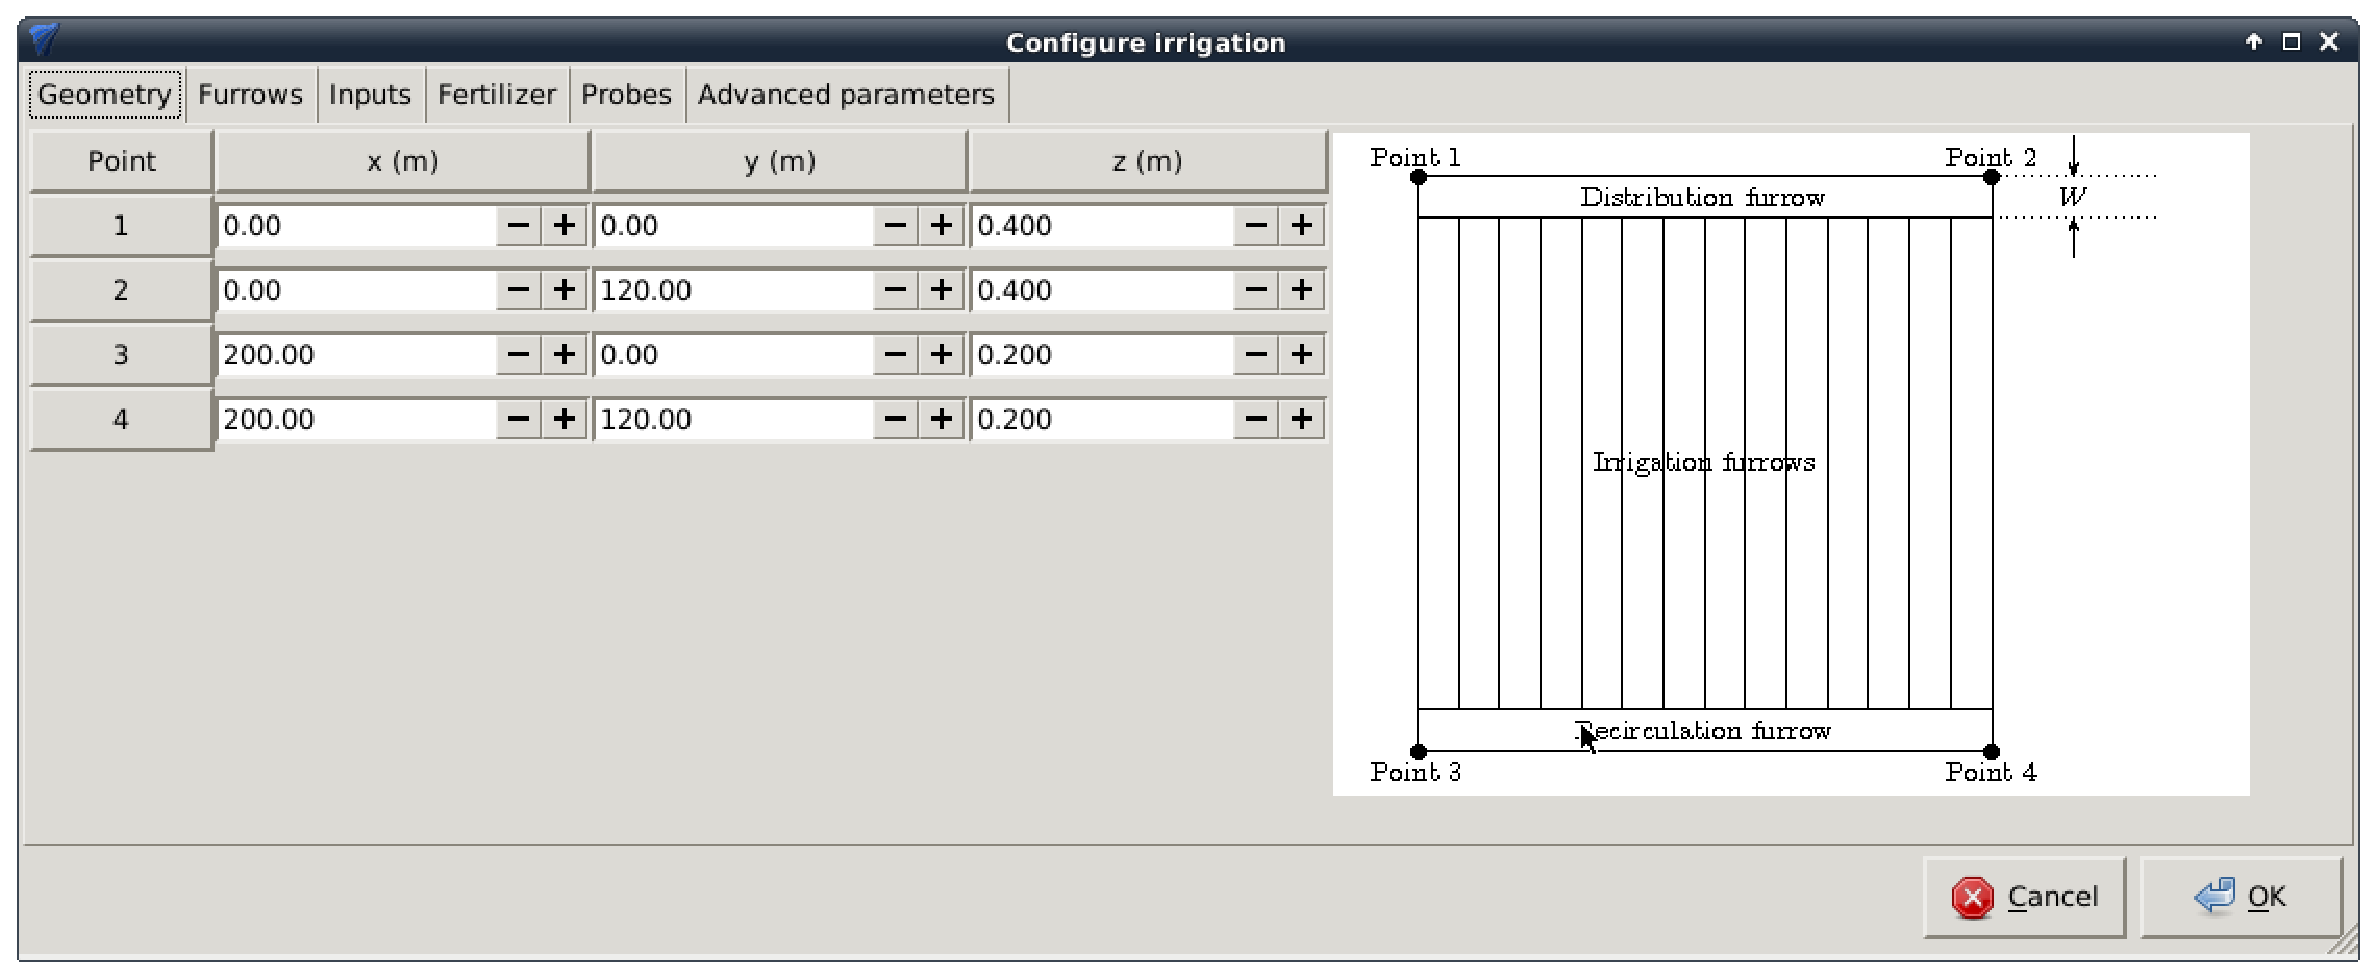
\includegraphics[width=1125\UNIT]{confGeomEN.eps}
\caption{Geometry configuration panel.}\label{geomWindow}
\end{center}
\end{figure}

As displayed in figure~\ref{geomWindow}, the distribution furrow runs between
points 1 and 2 and the recirculation furrow, if any, can be defined between
points 3 and 4. The irrigation furrows are assumed in the normal direction to
the former. In cases of isolated furrow only the distribution furrow between
points 1 and 2 is simulated.

\subsubsection{Furrow configuration panel}

\begin{figure}[!ht]
\begin{center}
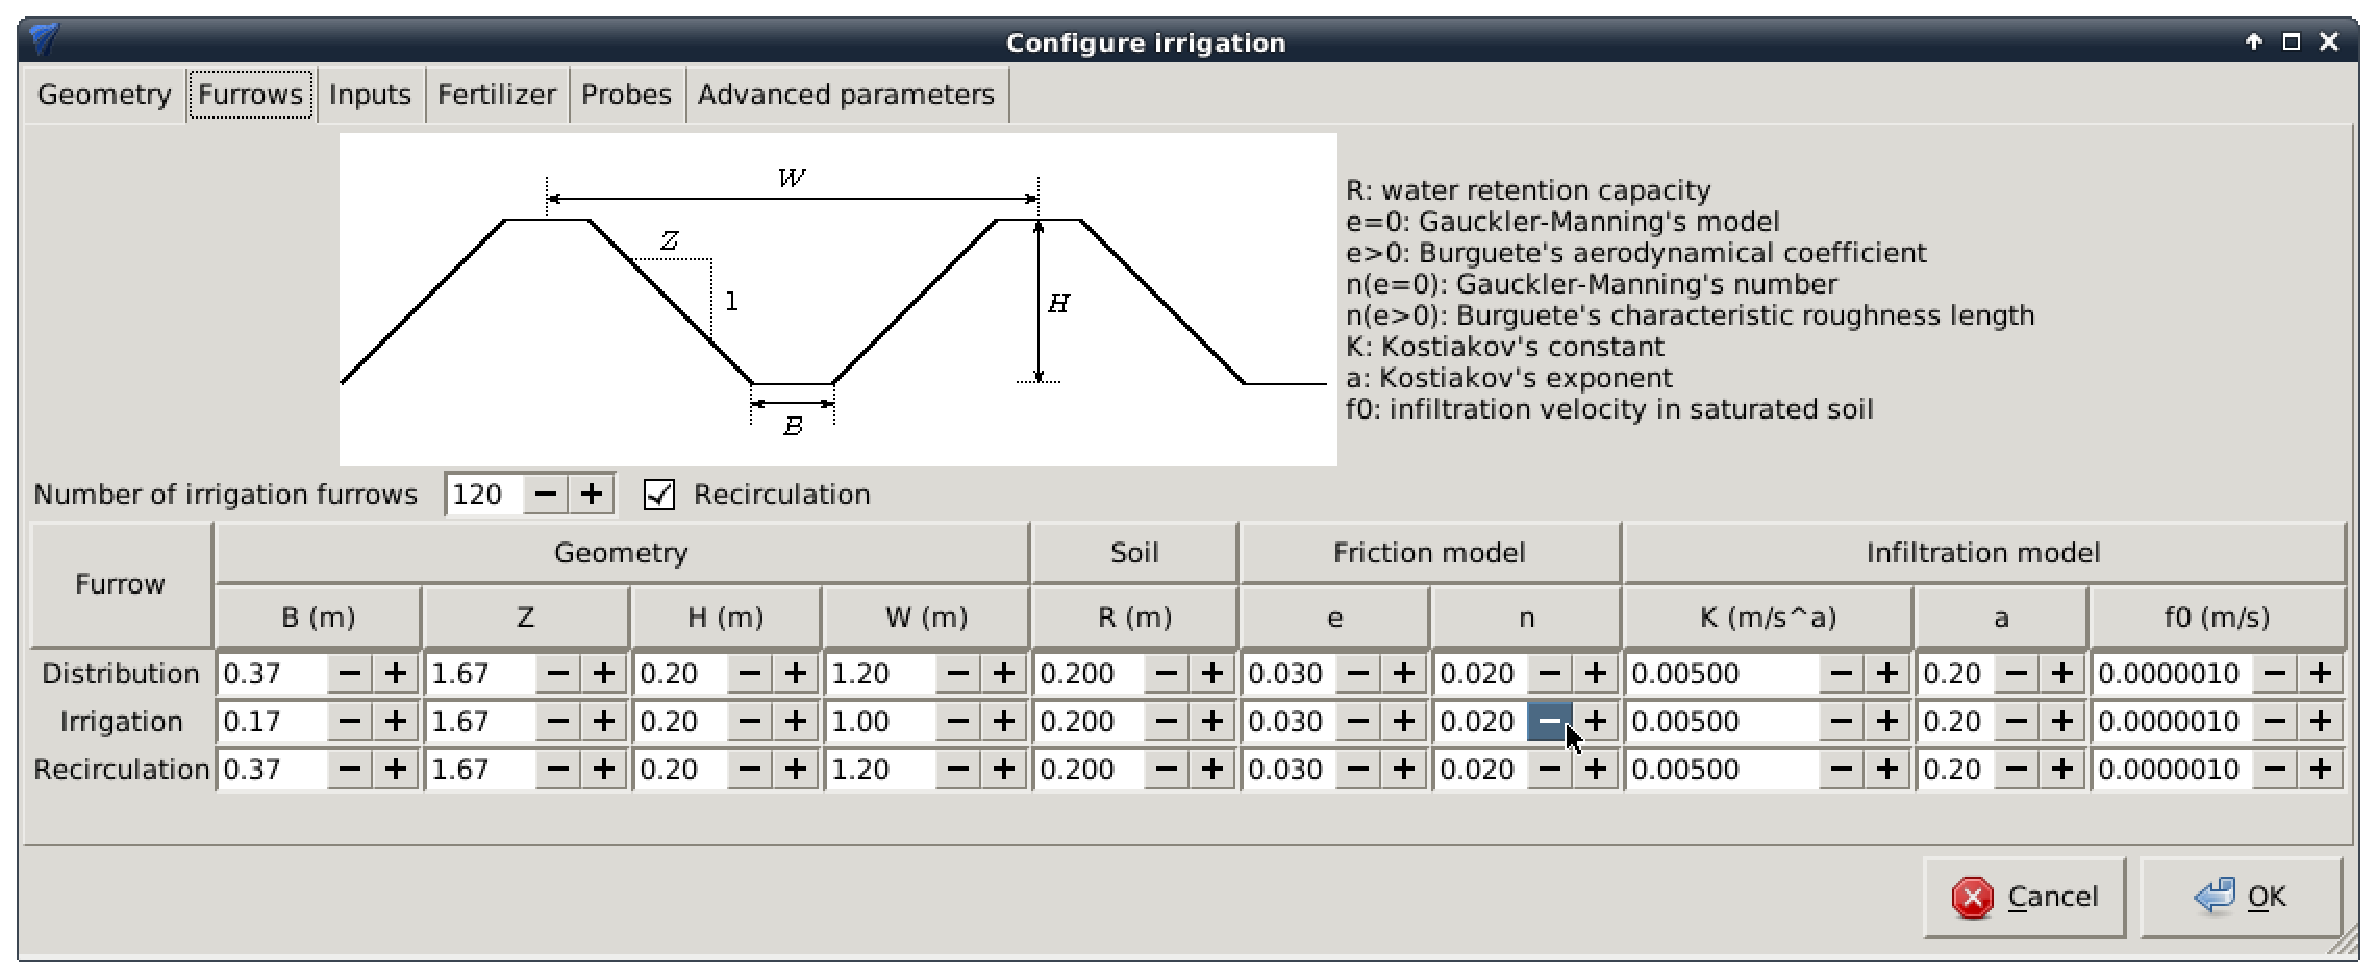
\includegraphics[width=1125\UNIT]{confSurcoEN.eps}
\caption{Furrow configuration panel.}\label{confSurcos}
\end{center}
\end{figure}

\begin{table}[!ht]\footnotesize
\centering
\caption{Furrow configuration panel parameters description.}\label{tabSurcos}
\begin{tabular}{ccl}
\hline
Parameter & Units & Description \\
\hline
$B$ & m & Base furrow width \\
$Z$ & - & Lateral furrow slope \\
$H$ & m & Furrow depth \\
$W$ & m & Distance between furrows \\
$R$ & m & Soil water retention capacity \\
$e>0$ & - & Burguete's bed aerodynamical coefficient \\
$e=0$ & - & Gauckler-Manning's model \\
$n$ (for $e>0$) & - & Burguete's characteristic roughness length \\ 
$n$ (for $e=0$) & s $\cdot$ m$^{-1/3}$ & Gauckler-Manning's number \\
$K$ & m $\cdot$ s$^{-a}$ & Kostiakov's constant \\
$a$ & - & Kostiakov's exponent \\
$f_0$ & m $\cdot$ s$^{-1}$ & Infiltration velocity in saturated soil \\
\hline
\end{tabular}
\end{table}

The panel displayed in figure~\ref{confSurcos} allows to define the geometric
properties of the furrows as divided in three types: distribution, recirculation
and irrigation furrows. The different options appear as active or inactive
depending on the previous definition of the furrow in our project. The available
characteristics to edit are all displayed in figure~\ref{confSurcos} and described in table~\ref{tabSurcos}. In cases
of isolated furrow simulations the number of irrigation furrows must be set to 0
and the furrow characteristics must be set at the distribution furrow.

\subsubsection{Inlet configuration panel}

The panel shown in figure~\ref{input} can be used to configure the total water
and fertilizer inlet to the furrow system. Every inlet is assigned to a location
point where the flow is applied, and is characterized by the initial and the
final application times of a constant discharge. Note that, if the point
assigned falls out of a furrow, the program finds the nearest position within a
furrow. The discharge is volumetric rate flow for the water and a mass flow rate
for the fertilizer. It is possible to define more complex inlet hydrographs by
means of a sequence of inlet discharges at the same point. 


\begin{figure}[!ht]
\begin{center}
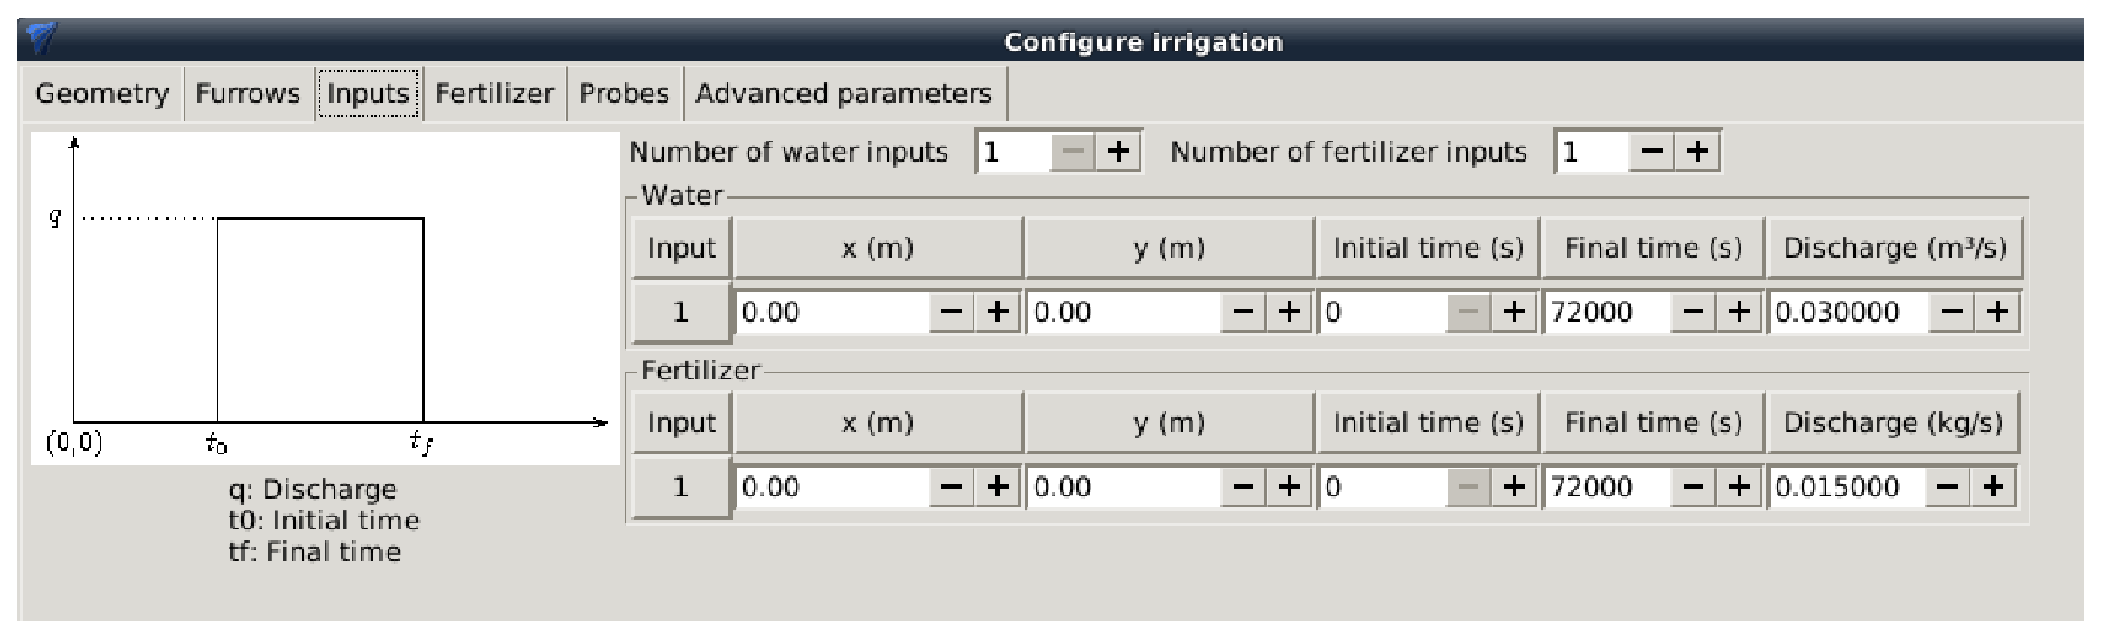
\includegraphics[width=993\UNIT]{confInputEN-2.eps}
\caption{Inlet configuration panel.}\label{input}
\end{center}
\end{figure}

\subsubsection{Fertilizer configuration panel}

The solubility characteristics of the fertilizer shown in
table~\ref{tabFertilizer} can be set here. Currently, only the instantaneous
solubility is considered.

\begin{table}[!ht]\footnotesize
\centering
\caption{Fertilizer configuration parameters.}\label{tabFertilizer}
\begin{tabular}{ccl}
\hline
Parameter & Units & Description \\
\hline
Solubility & kg $\cdot$ m$^{-3}$ & Instantaneous fertilizer solubility \\ 
\hline
\end{tabular}
\end{table}

\subsubsection{Probes configuration panel}

The panel displayed in figure~\ref{sondas} can be used to define the number of
probes and their location in the plot. Note that, if the point assigned falls
out of a furrow, the program finds the nearest position within a furrow.

\begin{figure}[!ht]
\begin{center}
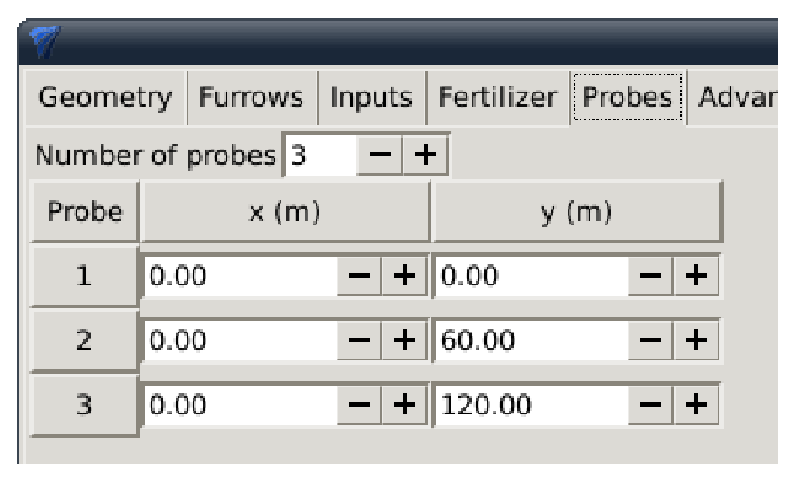
\includegraphics[width=366\UNIT]{confSondasEN-2.eps}
\caption{Probes configuration panel.}\label{sondas}
\end{center}
\end{figure}

\subsubsection{Advanced parameters configuration panel}

The panel shown in figure~\ref{param} contains advanced options to configure
the numerical simulation, as follows:

\begin{figure}[!ht]
\begin{center}
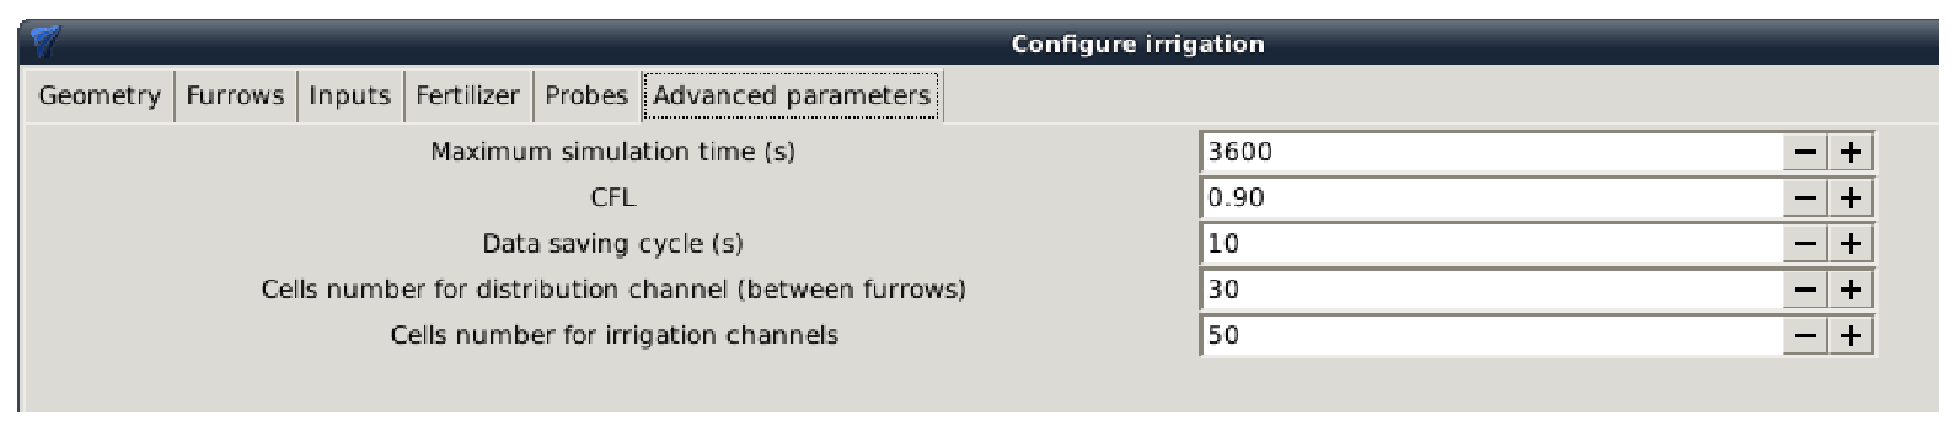
\includegraphics[width=923\UNIT]{confParamEN-2.eps}
\caption{Advanced parameters configuration panel.}\label{param}
\end{center}
\end{figure}

\begin{description}
\item{Maximum simulation time}: Usually, \emph{SURCOS} runs the
simulation from the initial conditions up to the moment all the applied water
has infiltrated in the terrain. In order to avoid excessively long simulation
times, this parameter can be used to state a horizon or target time. From that
limit, the computation stops even though some water still remains on the
surface.
\item{CFL}: Dimensionless numerical parameter proportional to the time step size
used by the resolution method. It takes values between 0 and 1 for numerical
stability reasons. Values close to 1 are optimal. Excessively low values can
slow the computation.
\item{Data saving cycle}: Simulation time interval used to save series of
numerical results in a file. It is possible to have $n=\frac{t_s}{p_v}$
snapshots of the irrigation event, with $t_s$ the simulation time and $p_v$ the
data saving cycle.  
\item{Cells number for distribution furrow (between irrigation furrows)}:
Number of computational cells in the distribution/recirculation furrow between
two irrigation furrows. A diagram can be shown in figure~\ref{FigMeshCells}. In
cases of isolated furrow this is the number of cells of the mesh.
\item{Cells number for irrigation furrows}: Number of computational cells
in every irrigation furrow. See an example in figure~\ref{FigMeshCells}. More
cells implies better quality in the results and slower computations.
\end{description}

\begin{figure}[ht!]
\centering
\begin{picture}(220,140)
	\put(70,130){Distribution furrow}
	\put(70,0){Recirculation furrow}
	\multiput(10,20)(0,100){2}{\line(1,0){200}}
	\multiput(10,20)(40,0){6}{\line(0,1){100}}
	\put(220,70){Irrigation}
	\put(220,60){furrows}
	\multiput(10,20)(10,0){5}{\multiput(0,0)(0,100){2}{\circle*{3}}}
	\multiput(130,20)(0,10){11}{\circle{3}}
	\put(60,65){Cell}
	\put(60,55){nodes}
	\put(85,65){\vector(1,0){40}}
	\put(70,75){\vector(-1,1){40}}
	\put(70,50){\vector(-2,-1){45}}

\end{picture}
\caption{Mesh example on a furrow network. This example has 6 irrigation
furrows, 5 cells at the distribution furrow between irrigation furrows
($\bullet$) and 11 cells at every irrigation furrow ($\circ$).
\label{FigMeshCells}}
\end{figure}

\subsection{Simulation}

After the configuration, the simulation of the project is performed by pressing
the button \emph{Execute} in the main menu.

\subsection{Results visualization}

\subsubsection{Graphical results}

A window showing a graphical plot of the numerical results can be accessed by
pressing the button \emph{Plot}.
It is possible to choose the furrow, the variable and the probe to view.
An interactive dial can be used to move forward and backward in time the
evolution of the variables represented in the graphics.
The program offers the possibility
to save the graphical results by pressing the button \emph{Save} at the bottom
of the window. The image of the plot appearing on the graphical window in that
moment, as the shown in next section in figures~\ref{evo1}-\ref{evoSonda}, is
saved in a \emph{png} format.

%\begin{figure}[!ht]
%\begin{center}
%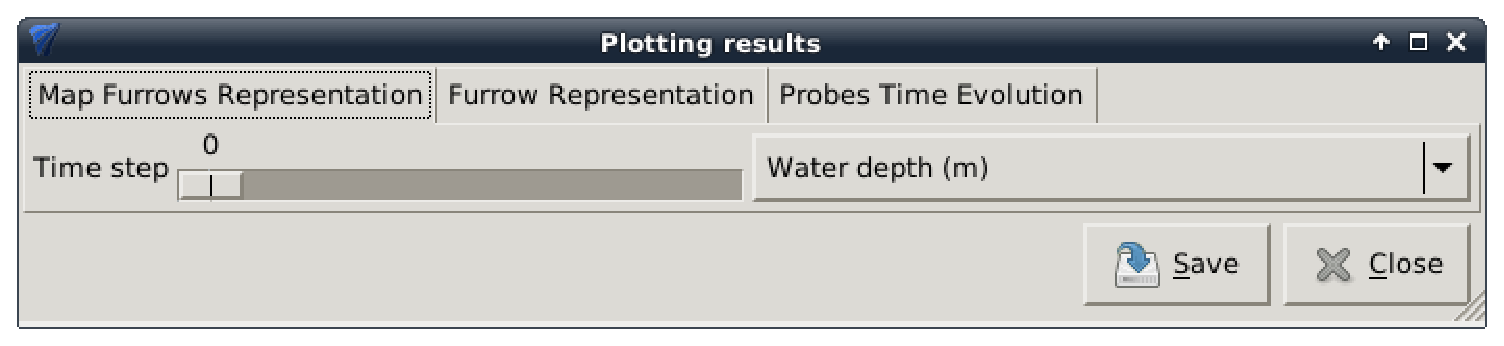
\includegraphics[width=706\UNIT]{menuRepresEN.eps}
%\caption{Plot selection window}\label{barraRepres}
%\end{center}
%\end{figure}

\emph{SURCOS} produces three types of plots. The first is a plan view of
the furrow network, with the possibility to display the distribution in the
network. The second graphical option is a Cartesian $xy$-plot of the
longitudinal profile along different furrows. The third graphical option is a
time evolution of the variables in the different probes. The variables that can
be plotted are those in table~\ref{tableVariables}.

\begin{table}[ht]\footnotesize
\caption{Variables to view on the plots.}
\label{tableVariables}
\begin{center}
\begin{tabular}{lcccc}
\hline
Variable & Units & Furrows & Furrow & Probe \\
& & network & profile & evolution\\
\hline
Surface water depth & m & x & x & x \\
Surface fertilizer concentration & kg~m$^{-3}$ & x & x & x \\
Infiltrated water volume & m$^2$ & x & x & - \\
\hspace{3mm} per unit furrow length \\
Infiltrated fertilizer mass & kg~m$^{-1}$ & x & x & - \\
\hspace{3mm} per unit furrow length \\
Discharge & m$^3$ s$^{-1}$ & - & x & - \\
Surface water volume & m$^2$ & - & x & - \\
\hspace{3mm} per unit furrow length \\
Surface fertilizer mass & kg~m$^{-1}$ & - & x & - \\
\hspace{3mm} per unit furrow length \\
Surface water and bed levels & m & - & x & - \\
Irrigation advance and recession times & s & - & x & - \\
\hline
\end{tabular}
\end{center}
\end{table}

Some examples of these graphics provided by the program are shown in the next
section (figures~\ref{evo1}-\ref{evoSonda}).

\subsubsection{Summary}

The access to the summary is through the button \emph{Summary}. This is useful
to produce a brief text report with the description of the irrigation
configuration and the most relevant results obtained. An example is displayed in
figure~\ref{wInforme}.

The results include the surface, infiltrated and percolated water and fertilizer
mass both in the irrigation furrows and in the distribution/recirculation
furrows. The infiltrated water mass in the soil remains available to the
crops by retention forces, contrary to the percolated water.

The uniformity of distribution of water ($UW_{25}$) and of the fertilizer
($UF_{25}$) follows the ratio between the infiltration average of the 25\% of
the less irrigated points and the total infiltration average:
\eq
{
	UW_{25}=\frac{\displaystyle\sum_{\alpha_i<25\%}\min\PA{\alpha_i,\,R_i\,W}}
		{\displaystyle\sum_i\min\PA{\alpha_i,\,R_i\,W}},\quad
	UF_{25}=\frac{\displaystyle
		\sum_{\phi_i<25\%}\min\PA{\phi_i,\,\frac{R_i\,W\,\phi_i}{\alpha_i}}}
		{\displaystyle\sum_i\min\PA{\phi_i,\,\frac{R_i\,W\,\phi_i}{\alpha_i}}},
}{EqUniformity}
with $R$ the water retention capacity of the soil. In furrow networks the
uniformity of distribution is calculated only in the irrigation furrows.

Finally, the efficiency is computed as the infiltrated mass in the irrigation
furrows divided by the total applied mass. Therefore, both the percolated mass
and the solid mass of solute, as well as the mass infiltrated in the
distribution/recirculation furrows in cases of furrow networks, are considered
losses in the estimation of the efficiency. 

\begin{figure}[!ht]
\begin{center}
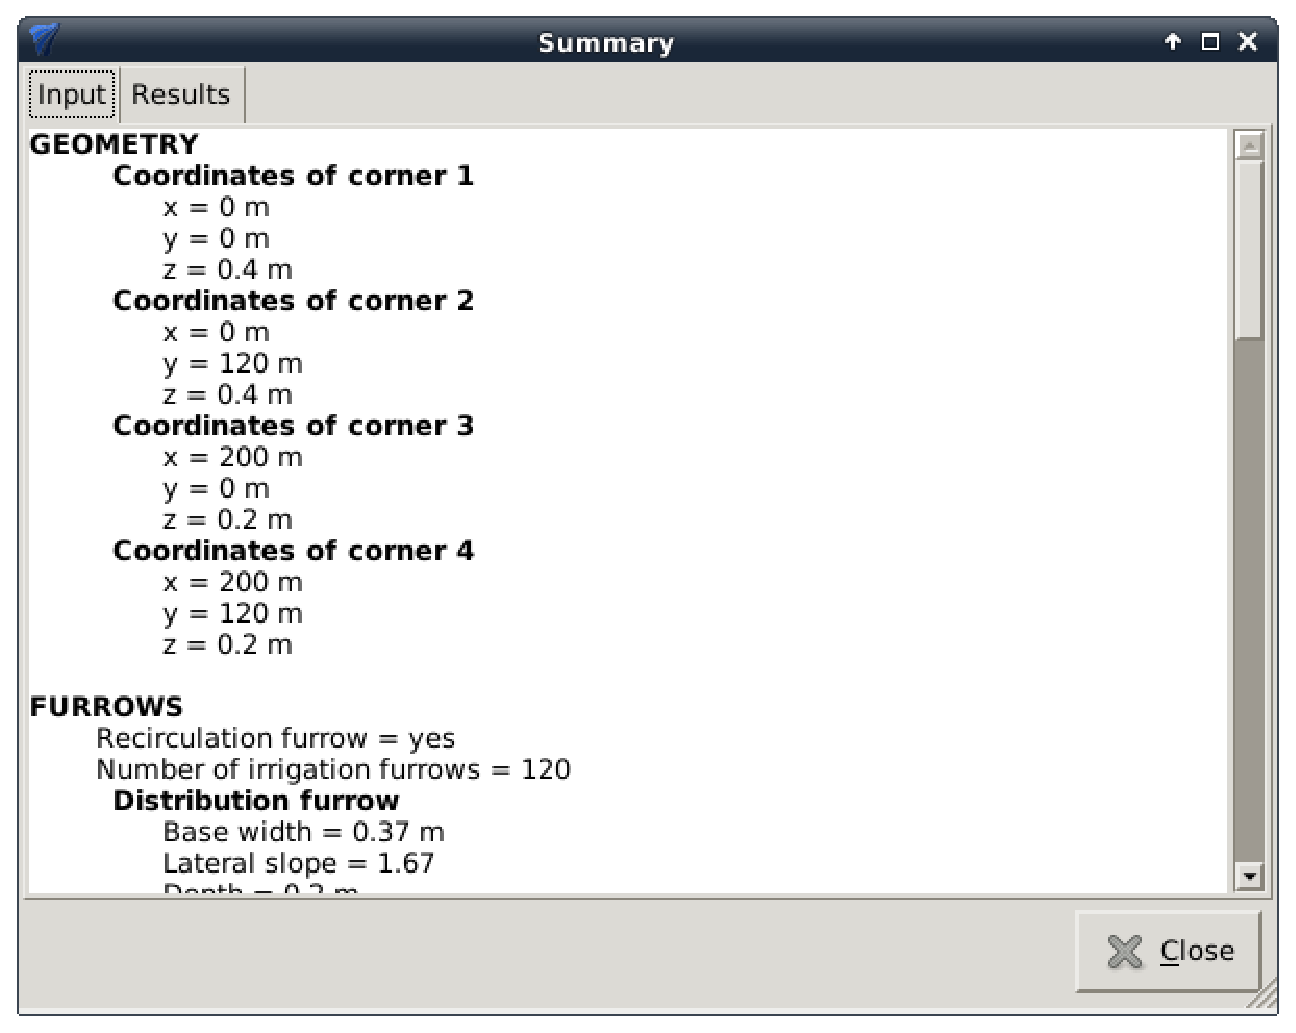
\includegraphics[width=606\UNIT]{sumarioEN.eps}
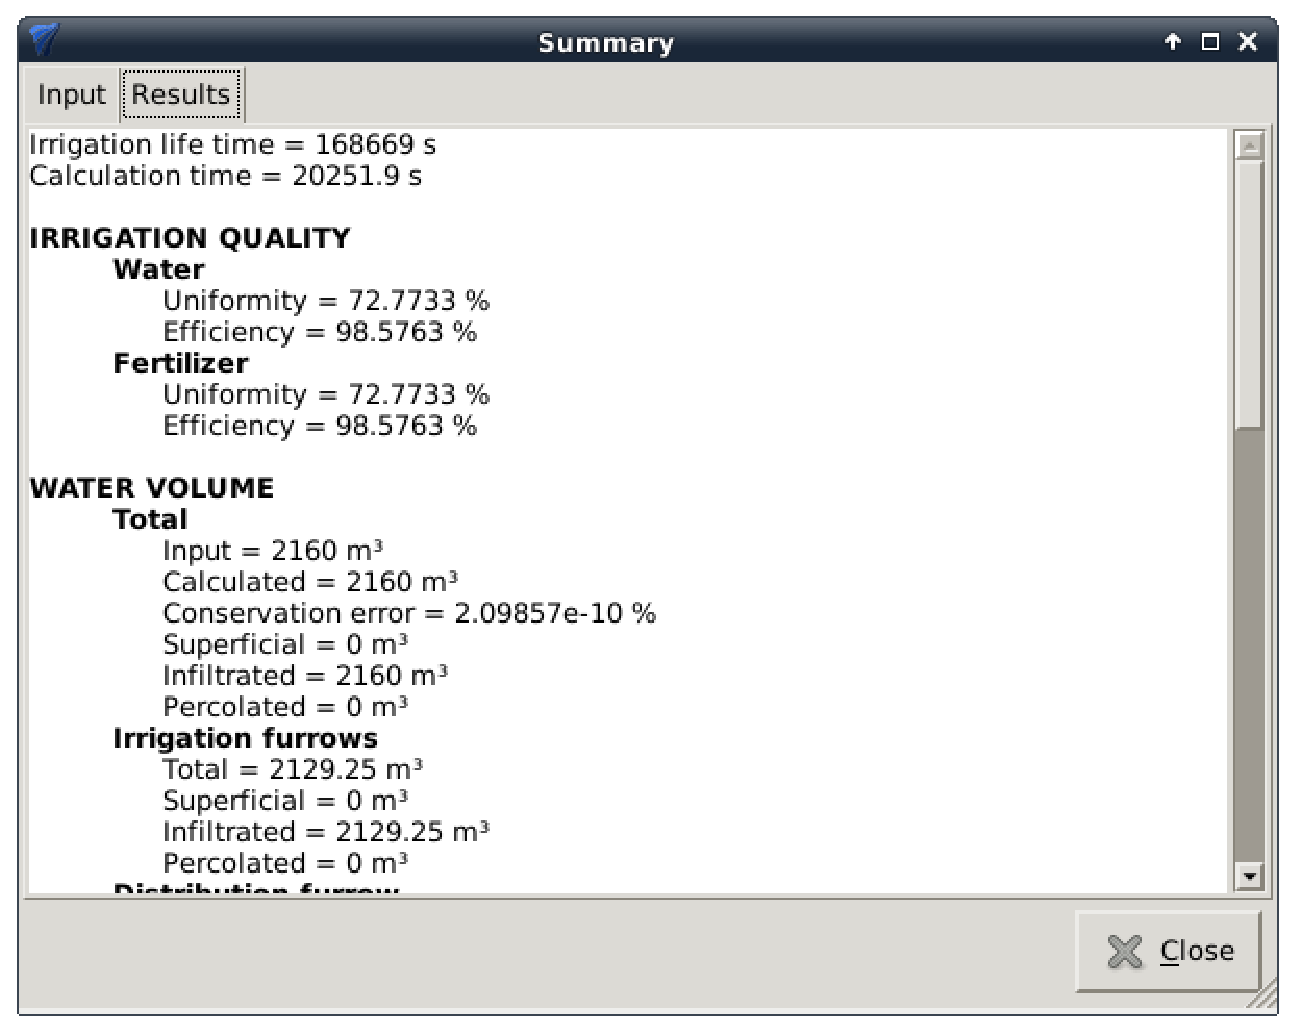
\includegraphics[width=606\UNIT]{sumario2EN.eps}
\caption{Summary of the input data (top) and results (bottom).}\label{wInforme}
\end{center}
\end{figure}

\section{Results}

This section is devoted to the presentation of examples of the numerical results
produced by the model in several scenarios of fertigation in furrows and furrow
networks. All the necessary input files for these examples can be downloaded
from \cite{Surcos} or \cite{SurcosGit}.

\subsection{Simulation of 9 fertigation scenarios in a level isolated furrow}

A single zero slope furrow with total length 30~m is first presented. The
furrow cross section is trapezoidal with $B_0=0.17$~m, $Z=1.2$, $H=0.27$~m and
$W=1$~m. A low retention capacity soil (0.06~m) is assumed with a roughness 
Gauckler-Manning $n=0.015$~m~s$^{-1/3}$ and infiltration parameters
$K=0.0032$~m~s$^{-a}$, $a=0.42$ and $f_0=0$~m~s$^{-1}$.
The water inlet point is located at the upstream end ($l=0$~m) whereas the
fertilizer inlet point is assumed at $l=1$~m. In all the scenarios 0.9~m$^3$ of
water are applied as well as 0.9~kg of fertilizer with a solubility
$S=10$~kg~m$^{-3}$. The fertilizer is applied at a constant rate but during
application times of different duration. The final irrigation time ($t_s$) used
is the one required for the total infiltration of the surface water. The
discretization parameters are the grid size $\delta l=1$~m and the time step
that is ruled by the $\mathrm{CFL}=0.9$ in all the simulations. The
computational time spent in the 9 scenarios has been 0.37~s on a desktop PC with
Intel Core i5 3.2 GHz processor without any parallelization.

Table~\ref{TabFurrow} contains the detail of the different inlet discharge
values as well as the initial ($t_i$) and final ($t_f$) application times. The
final irrigation time and the distribution uniformity results are also included.
Figure~\ref{FigCases} is the plot of the longitudinal profile of infiltrated
water and solute. Better uniformity values are obtained with larger inlet
discharges. The application of the fertilizer 1~m away from the water inlet
point reduces the fertilizer uniformity as the fertilizer infiltration upstream
the application point is negligible. The distributed fertilizer application
strategies (in scenarios 2, 5 an 8 it is applied during the first half-period
whereas in scenarios 3, 6 and 8 it is applied during the second half-period) reduce
considerably the fertilizer uniformity in general.

\begin{table}[ht!]
\centering
\caption{Final irrigation time, discharges, application times and
water/fertilizer uniformity for scenarios 1-9.\label{TabFurrow}}
\footnotesize
\begin{tabular}{|c|c|cccc|cccc|}
\hline
&&\multicolumn{4}{|c|}{Water}&\multicolumn{4}{|c|}{Fertilizer}\\
\hline
Scenario&$t_s$&$Q_{in}$&$t_i$&$t_f$&$UW_{25}$&$Q_{in}$&$t_i$&$t_f$&$UF_{25}$\\
&s&m$^3$~s$^{-1}$&s&s&\%&kg~s$^{-1}$&s&s&\%\\
\hline
1&1020&0.002&0&450&88.72&0.002&0&450&65.43\\
2&1020&0.002&0&450&88.72&0.004&0&225&42.39\\
3&1020&0.002&0&450&88.72&0.004&225&450&68.42\\
4&858&0.005&0&180&95.37&0.005&0&180&71.85\\
5&858&0.005&0&180&95.37&0.010&0&90&59.31\\
6&858&0.005&0&180&95.37&0.010&90&180&22.12\\
7&830&0.010&0&90&96.58&0.010&0&90&71.69\\
8&830&0.010&0&90&96.58&0.020&0&45&54.22\\
9&830&0.010&0&90&96.58&0.020&45&90&5.26\\
\hline
\end{tabular}
\end{table}

\begin{figure}[ht!]
\centering
\begin{minipage}{0.49\textwidth}
\centering
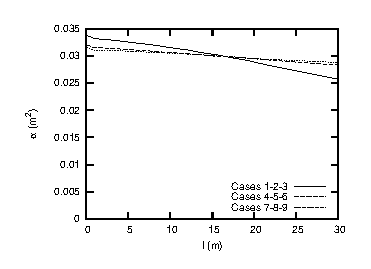
\includegraphics{water1-9.eps}
(a)
\end{minipage}
\begin{minipage}{0.49\textwidth}
\centering
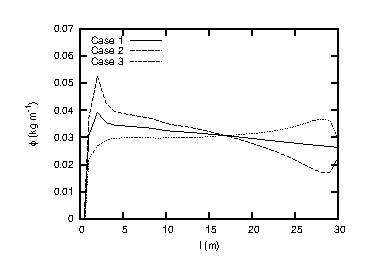
\includegraphics{fertilizer123.eps}
(b)
\end{minipage}
\begin{minipage}{0.49\textwidth}
\centering
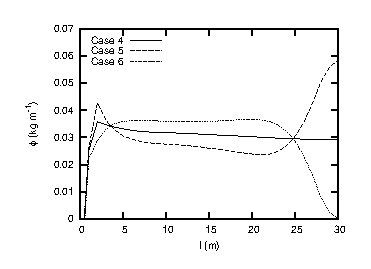
\includegraphics{fertilizer456.eps}
(c)
\end{minipage}
\begin{minipage}{0.49\textwidth}
\centering
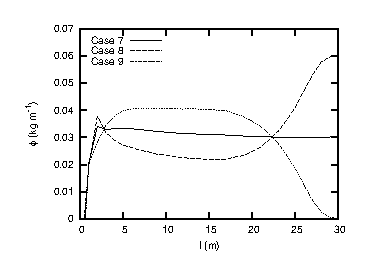
\includegraphics{fertilizer789.eps}
(d)
\end{minipage}
\caption{Longitudinal profiles of volume of water (a) and mass of solute
(b, c and d) infiltrated per unit length of furrow for the scenarios 1-9.}
\label{FigCases}
\end{figure}

\subsection{Simulation of 12 fertigation scenarios in a furrow network}

This set of scenarios (10 to 21) is concerned with the simulation in a plot
120~m~x~200~m with a network of 120 irrigation furrows. A low infiltration soil
with the Kostiakov-Lewis parameters $K=1.0\cdot10^{-3}$~m~s$^{-a}$,
$a=0.2$ and $I_c=1.0\cdot10^{-6}$~m~s$^{-1}$ is assumed. The roughness model (\ref{EqSf})
has been used with the typical  furrow values $\epsilon=0.03$ and $d=0.02$~m.
The irrigation furrows are assumed of trapezoidal cross section given by 
$B_0=0.17$~m, $Z=1.67$, $H=0.20$~m, $W=1$~m and with a longitudinal slope $S_0=0.0001$.
Level distribution and recirculation furrows are assumed ($S_0=0$) with a
cross section given by $B_0=0.37$~m, $Z=1.67$, $H=0.25$~m and $W=1.2$~m. A total
water volume of 2160~m$^3$ and 1080~kg fertilizer with solubility
$S=1$~kg~m$^{-3}$ are applied during 20 hours. In scenarios 10-13 water is applied at
an extreme point in the distribution furrow. In scenarios 14-17 it is applied at
the mid-point of the distribution furrow and in scenarios 18-21 water is applied
simultaneously at the two end points of the distribution furrow. On the other
hand, in scenarios 10, 14 and 18 the fertilizer is applied during 20 hours, in
scenarios
11, 15 and 19 it is applied during the first 10 hours and in scenarios 12, 16 and
20 it is applied in the last 10 hours. In all scenarios, water and fertilizer
are applied at the same location except in scenarios 13, 17 and 21, where the
fertilizer is applied suddenly at the beginning time on 9 equally distributed
points along the distribution furrow. Figures~\ref{FigNetworkWater}
and~\ref{FigNetworkFertilizer}, and table~\ref{TabNetwork}, show the sketch of
the water and fertilizer application in the different scenarios.

\begin{figure}[ht!]
\centering
\begin{picture}(320,100)
\put(0,90){\small Distribution furrow}
\put(15,85){\vector(1,-2){10}}
\multiput(30,30)(100,0){3}
{
	\multiput(0,0)(0,2){28}{\line(1,0){90}}
	\multiput(0,0)(90,0){2}{\line(0,1){54}}
}
\put(30,30){\circle*{4}}
\put(0,10){\small Water inlet}
\put(15,20){\vector(3,2){10}}
\put(130,57){\circle*{4}}
\put(230,30){\circle*{4}}
\put(230,84){\circle*{4}}
\put(50,0){Scenarios 10-13}
\put(140,0){Scenarios 14-17}
\put(240,0){Scenarios 18-21}
\end{picture}
\caption{Water application in scenarios 10-21.
\label{FigNetworkWater}}
\end{figure}

\begin{figure}[ht!]
\centering
\begin{picture}(260,200)
\put(0,190){\small Distribution furrow}
\put(15,185){\vector(1,-2){10}}
\multiput(30,30)(0,100){2}
{
	\multiput(0,0)(140,0){2}
	{
		\multiput(0,0)(0,2){28}{\line(1,0){90}}
		\multiput(0,0)(90,0){2}{\line(0,1){54}}
	}
}
\put(30,130){\circle{4}}
\put(0,110){\small Fertilizer inlet}
\put(15,120){\vector(3,2){10}}
\put(170,157){\circle{4}}
\put(30,30){\circle{4}}
\put(30,84){\circle{4}}
\multiput(170,30)(0,6.75){9}{\circle{4}}
\put(50,100){Scenarios 10-12}
\put(180,100){Scenarios 14-16}
\put(40,0){Scenarios 18-20}
\put(160,0){Scenarios 13, 17 and 21}
\end{picture}
\caption{Fertilizer application in scenarios 10-21.
\label{FigNetworkFertilizer}}
\end{figure}

\begin{table}[ht!]
\centering
\caption{Water and fertilizer applications for scenarios 10-21.
\label{TabNetwork}}
\footnotesize
\begin{tabular}{|c|cccc|cccc|}
\hline
&\multicolumn{4}{|c|}{Water}&\multicolumn{4}{|c|}{Fertilizer}\\
\hline
Scenario&$t_i$&$t_f$&Inlets&Inlets&$t_i$&$t_f$&Inlets&Inlets\\
&h&h&number&location&h&h&number&location\\
\hline
10&0&20&1&Corner&0&20&1&Corner\\
11&0&20&1&Corner&0&10&1&Corner\\
12&0&20&1&Corner&10&20&1&Corner\\
13&0&20&1&Corner&\multicolumn{2}{c}{Suddenly at $t=0$}&9&Distributed\\
14&0&20&1&Middle&0&20&1&Middle\\
15&0&20&1&Middle&0&10&1&Middle\\
16&0&20&1&Middle&10&20&1&Middle\\
17&0&20&1&Middle&\multicolumn{2}{c}{Suddenly at $t=0$}&9&Distributed\\
18&0&20&2&Corners&0&20&2&Corners\\
19&0&20&2&Corners&0&10&2&Corners\\
20&0&20&2&Corners&10&20&2&Corners\\
21&0&20&2&Corners&\multicolumn{2}{c}{Suddenly at $t=0$}&9&Distributed\\
\hline
\end{tabular}
\end{table}

In all cases, the total irrigation lifetime required by complete infiltration of
surface water takes about 46-47 hours. For the numerical simulation, a grid
spacing $\delta l=1$~m was used in all scenarios, leading to 24480 cells. The
time step was controlled by $\mathrm{CFL}=0.9$.

Figure~\ref{evo1} shows a snapshot of the program with a distribution map of the
surface water depth in scenario 10 at $t=43200$~s.

\begin{figure}[!ht]
\begin{center}
%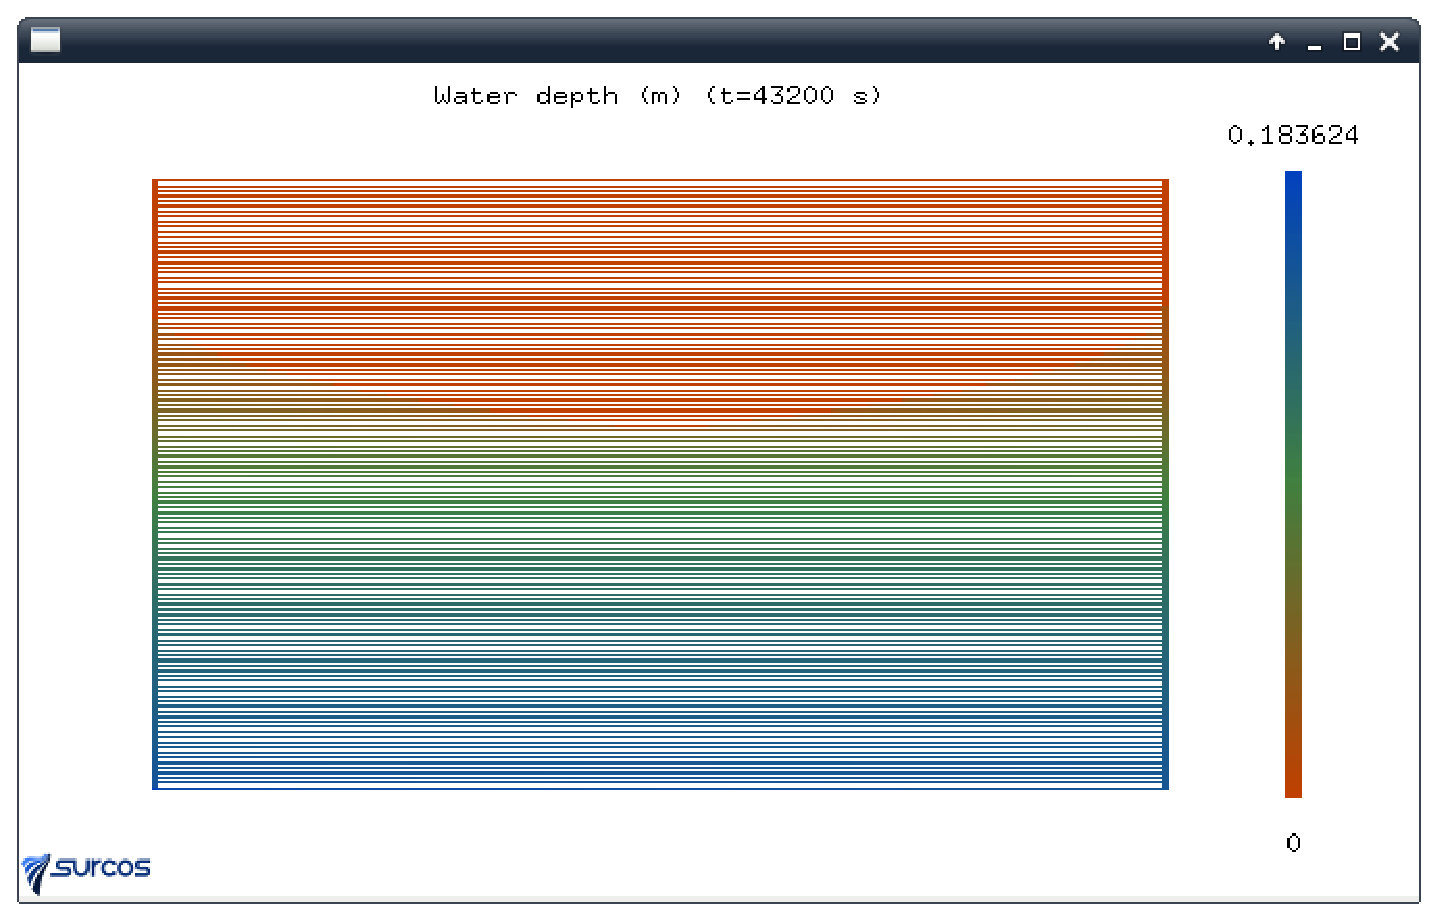
\includegraphics[width=674\UNIT]{evo1EN.eps}
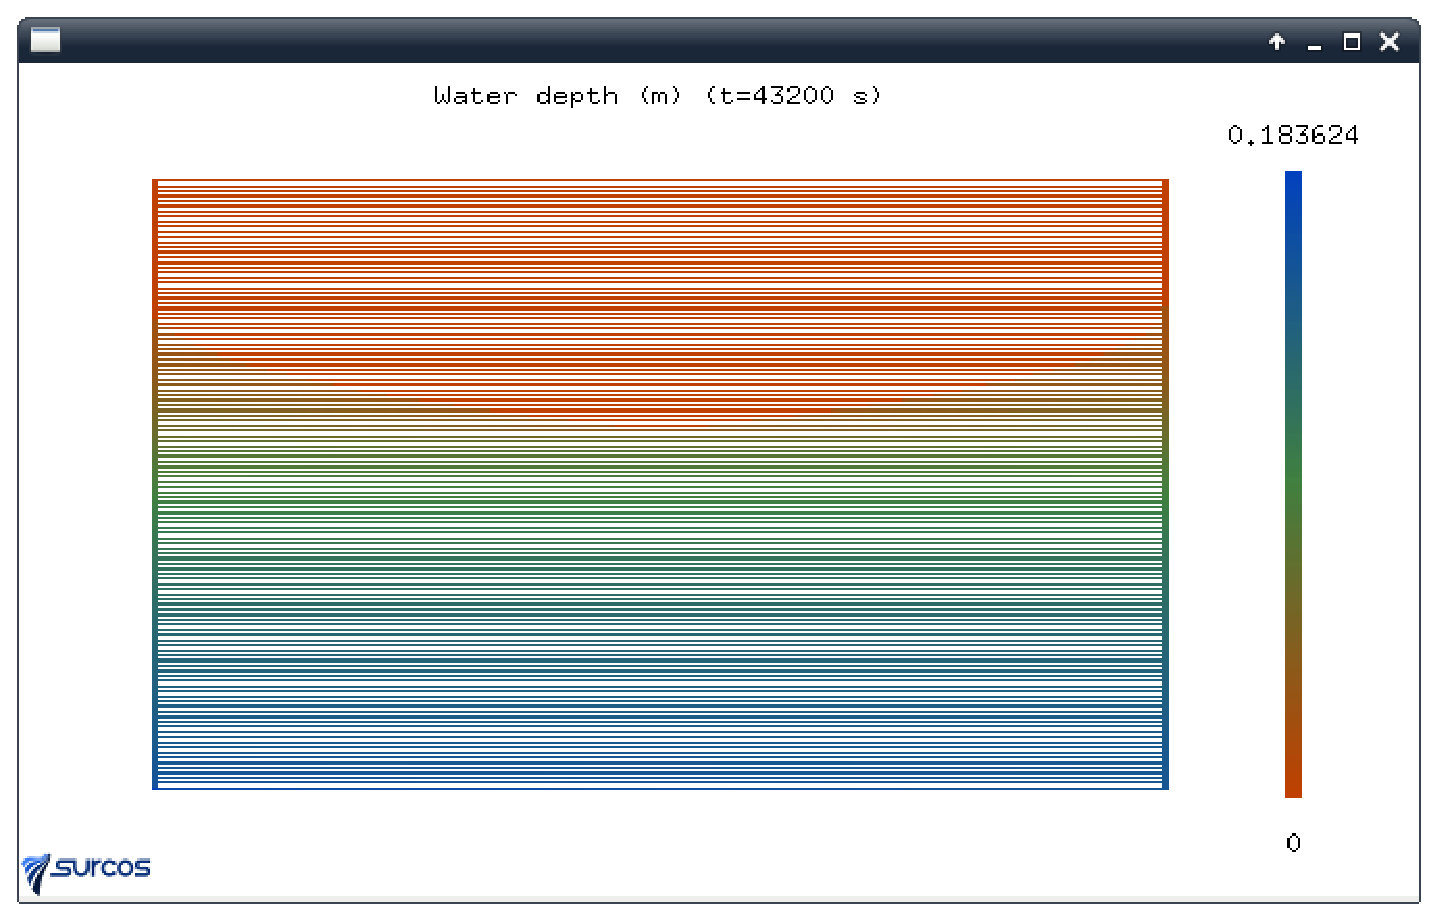
\includegraphics[width=\textwidth]{evo1EN.eps}
\caption{Map of the water depth for scenario 10 at
$t=43200$~s as displayed by \emph{SURCOS}.}\label{evo1}
\end{center}
\end{figure}

Figure~\ref{evo2} shows a snapshot of the program with the longitudinal surface
and infiltrated water depth profiles in the 60th furrow for scenario 10 at
$t=3240$~s.

\begin{figure}[ht!]
\begin{center}
%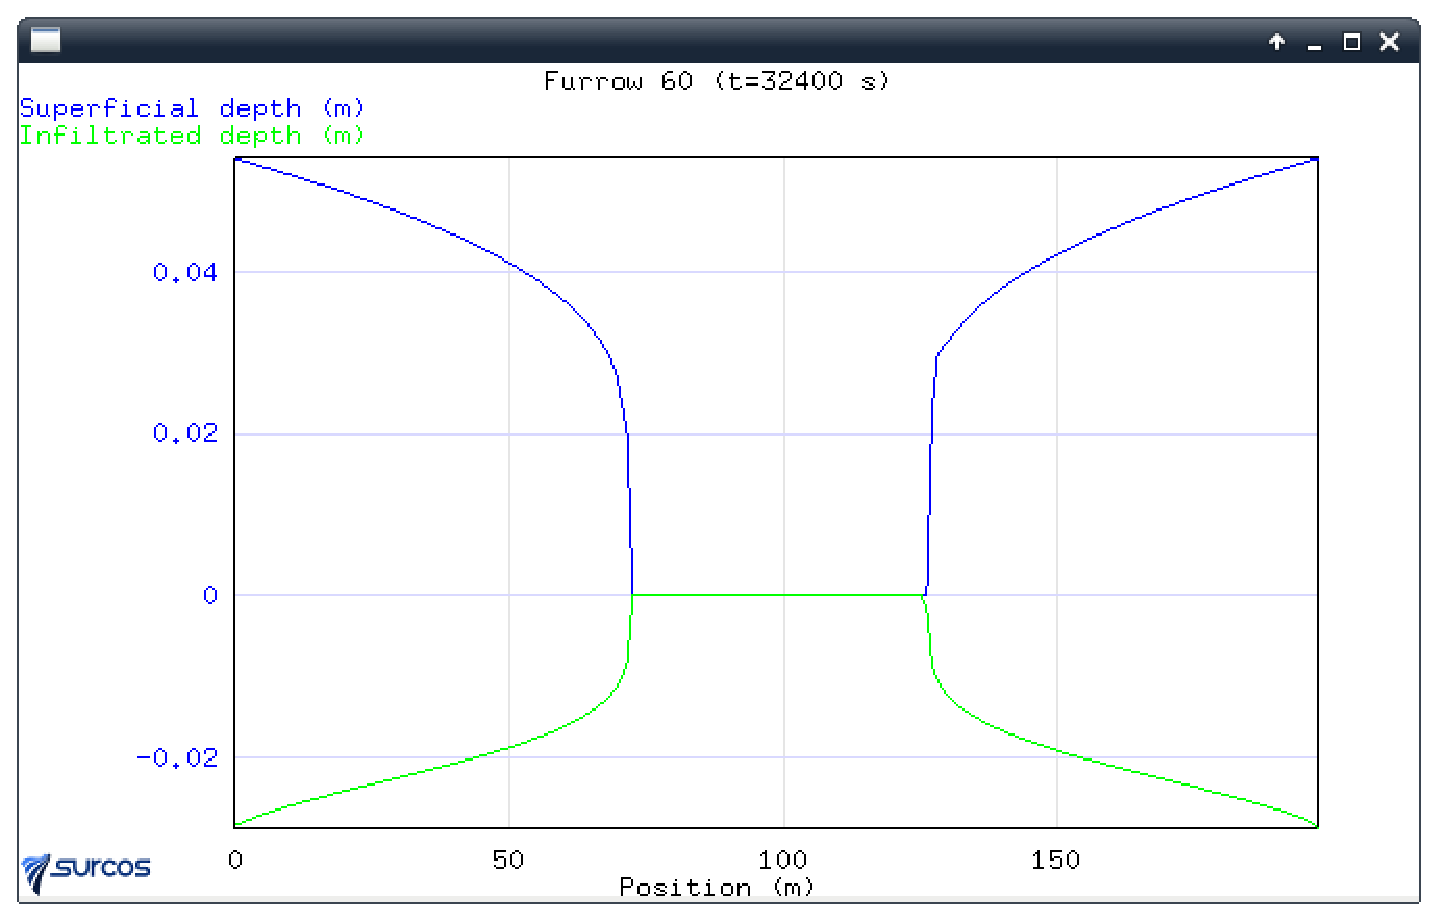
\includegraphics[width=674\UNIT]{evoSurcoEN.eps}
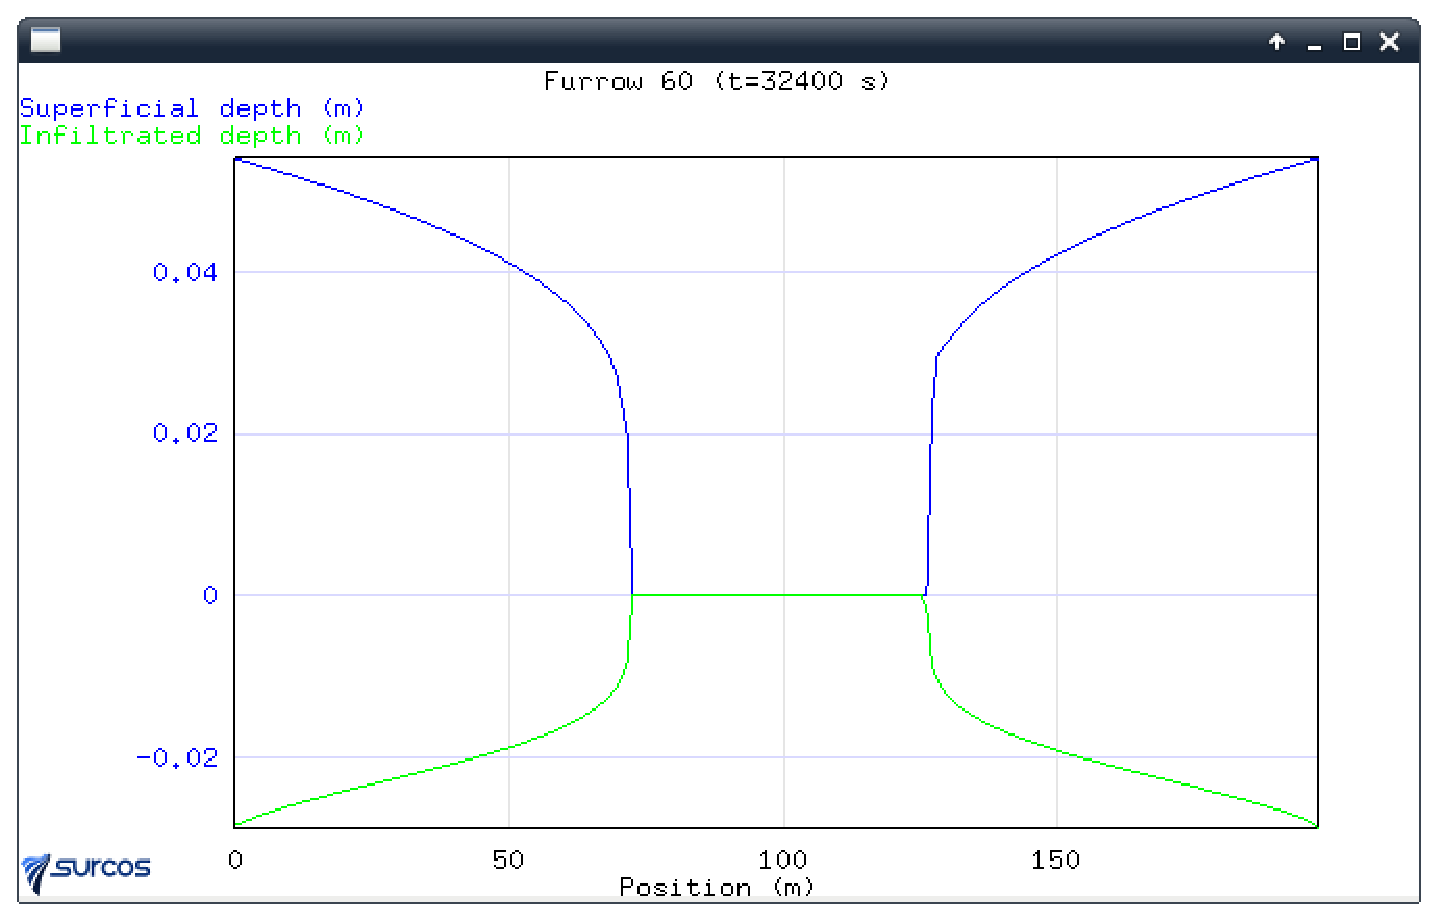
\includegraphics[width=\textwidth]{evoSurcoEN.eps}
\caption{Longitudinal profile of the surface and infiltrated
water in the 60th irrigation furrow for the scenario 10 at $t=32400$~s displayed by
\emph{SURCOS}.}\label{evo2}
\end{center}
\end{figure}

Figure~\ref{evoSonda} shows a snapshot of the program with the time evolution of
the surface water depth and concentration at a point located in the mid point of
the distribution furrow for scenario 10. 
\begin{figure}[ht!]
\begin{center}
%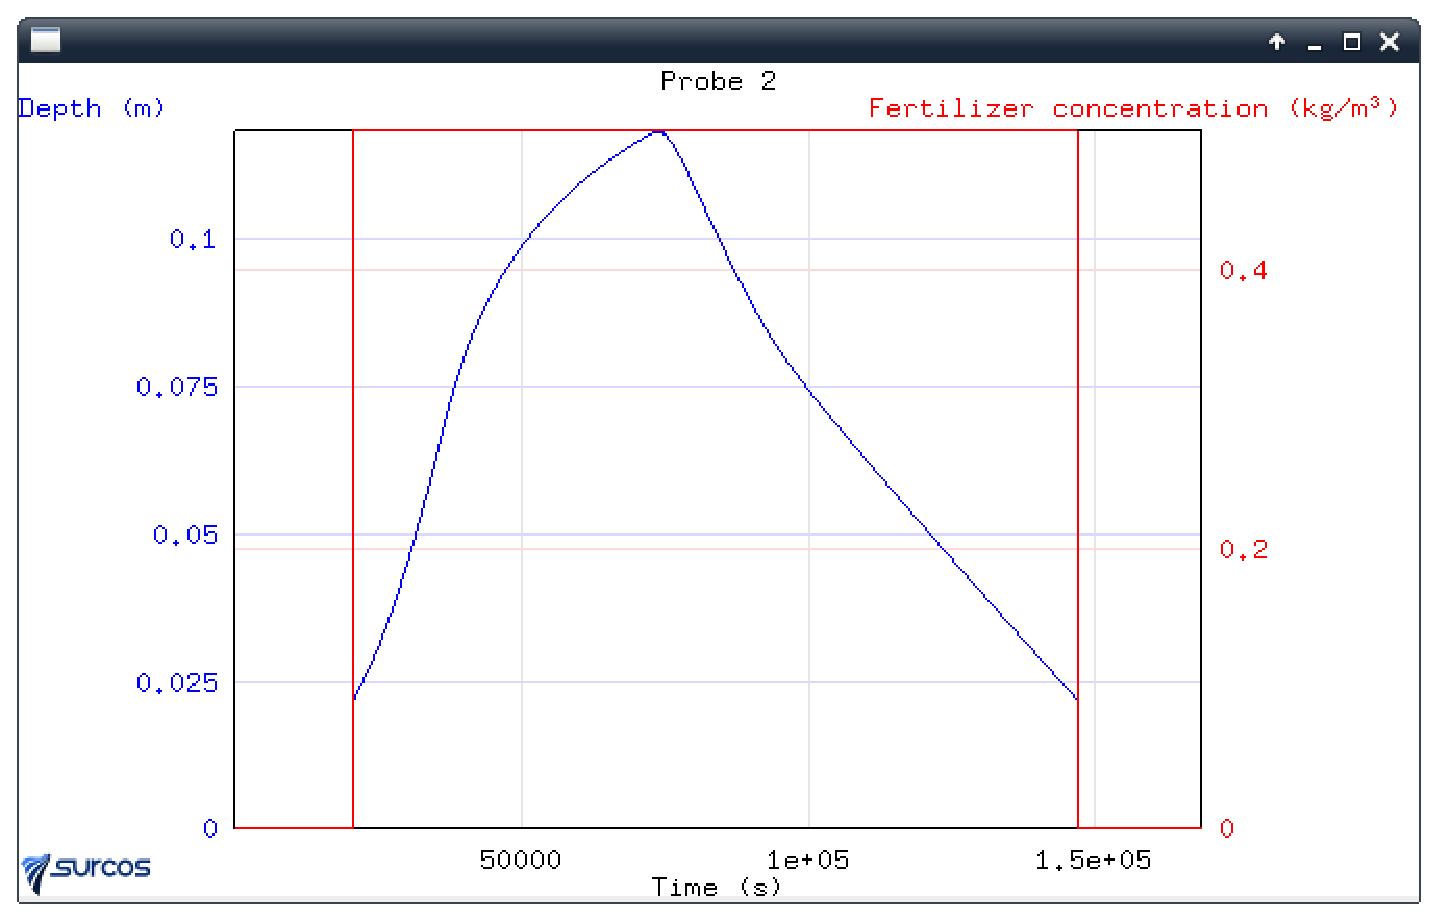
\includegraphics[width=674\UNIT]{evoSondaEN.eps}
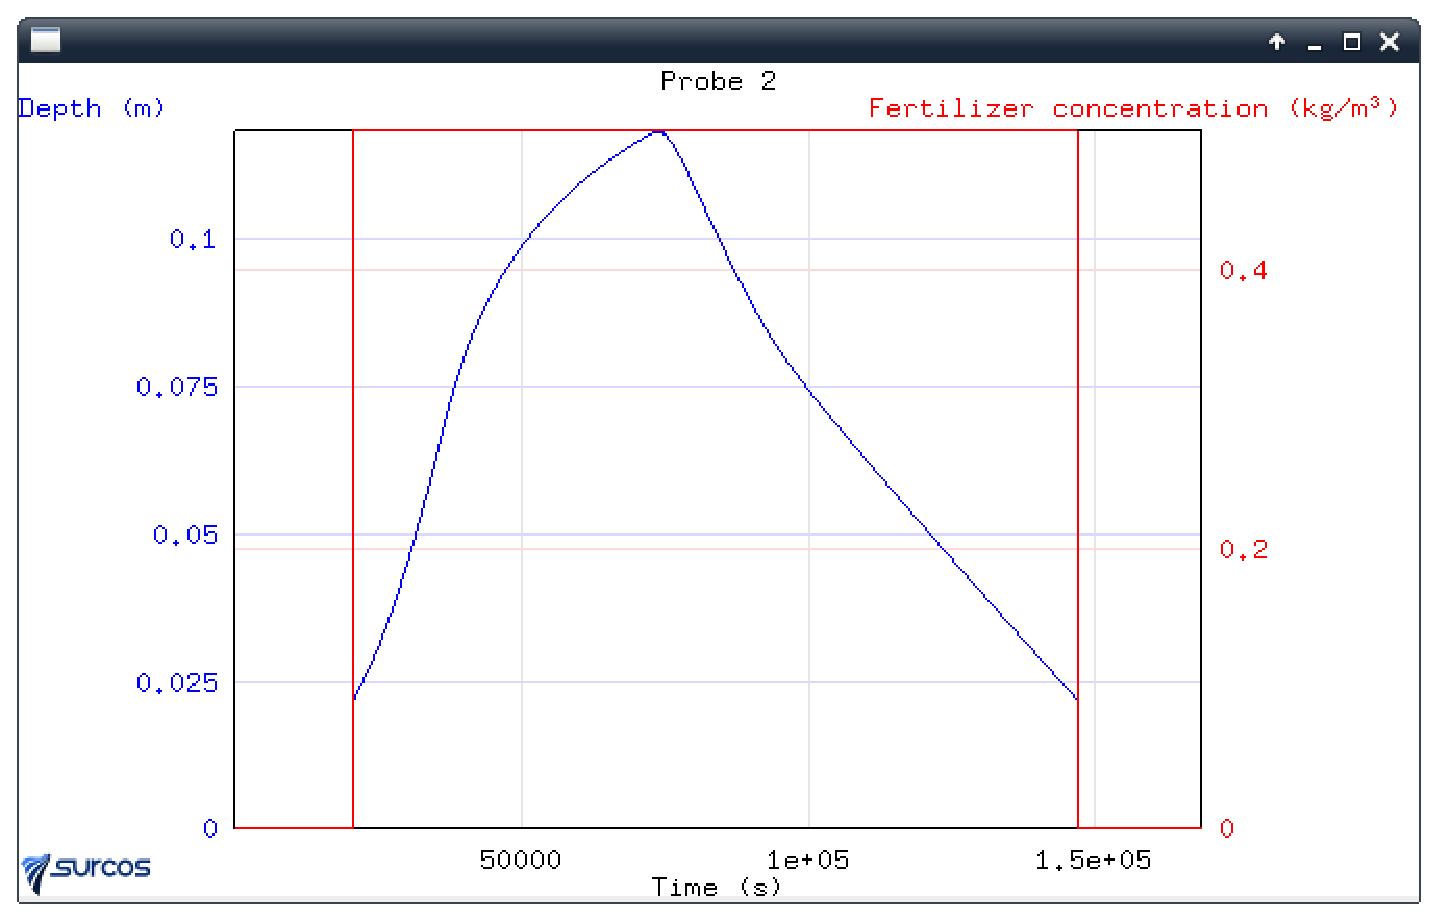
\includegraphics[width=\textwidth]{evoSondaEN.eps}
\caption{Time evolution at a probe located at the center of the distribution
furrow for scenario 10 as displayed by \emph{SURCOS}.}\label{evoSonda}
\end{center}
\end{figure}

Table~\ref{TabFurrowNetwork} presents the irrigation times as well as water and
fertilizer efficiency and uniformity achieved for scenarios 10-21.  The water application efficiency is excellent in all cases, with a
zero percolation flow. The fertilizer application efficiency is also excellent
except in scenarios 13, 17 and 21 where some of the fertilizer is not dissolved. 
The water distribution uniformity is good ($>76\%$) and improves when the inlet
is located at the distribution furrow midpoint or end points ($\approx 87\%$).
The fertilizer distribution uniformity is also good when it is applied together
with water (scenarios 10, 14 and 18). The fractional application of the fertilizer in
the first or second half of the application time reduces the uniformity. It is
worth noting that the strategy of spatial fertilizer distribution along 9 points
in the distribution furrow not only reduces efficiency, due to the non-dissolved
solid fraction, but also produces a loss in uniformity in these scenarios.

\begin{table}[ht!]
\centering
\caption{Final irrigation times as well as water and fertilizer
efficiency and uniformity achieved for scenarios 10-21.\label{TabFurrowNetwork}}
\footnotesize
\begin{tabular}{|c|c|cc|cc|}
\hline
&&\multicolumn{2}{|c|}{Water}&\multicolumn{2}{|c|}{Fertilizer}\\
\hline
Scenario&$t_s$&$EW$&$UW_{25}$&$EF$&$UF_{25}$\\
&hh:mm&\%&\%&\%&\%\\
\hline
10&46:39&98.58&76.86&98.58&\bf 76.86\\
11&46:39&98.58&76.86&98.91&4.77\\
12&46:39&98.58&76.86&98.01&10.33\\
13&46:39&98.58&76.86&74.47&1.81\\
14&46:19&98.55&87.37&98.55&\bf 87.37\\
15&46:19&98.55&87.37&98.78&34.08\\
16&46:19&98.55&87.37&98.31&33.63\\
17&46:19&98.55&87.37&65.51&0.97\\
18&46:19&98.55&87.34&98.55&\bf 87.34\\
19&46:19&98.55&87.34&98.79&33.27\\
20&46:19&98.55&87.34&98.14&32.90\\
21&46:19&98.55&87.34&74.13&0.22\\
\hline
\end{tabular}
\end{table}

The time used by a 2.8 GHz Intel Core i7 desktop computer to run the 12
scenarios in four parallel processes, in order to do an optimal use of the four
CPU cores, was 14~h~:~02~min, about one hour per simulation.

\section{Conclusions}

This work has presented \emph{SURCOS}. The core of the program is a well
tested mathematical model including shallow water flow and solute transport
solved using a second order TVD scheme. The verification and validation of the
numerical model can be found in previous publications
\citep{JaviSurcos1,JaviSurcos2}. The model is adapted to furrow fertigation and
implements an infiltration equation that automatically adjusts to variations in
the wetted perimeter, a roughness equation based on an absolute roughness
parameter, and an equation for the estimation of the longitudinal diffusion
parameter. The model also incorporates a specific treatment of the boundary
conditions formulated to ensure perfect global mass conservation. The model goes
beyond furrow irrigation and fertigation to furrow networks by means of a simple
and computationally efficient approach to the junction conditions, considered as
internal boundaries.

Numerical tests have been used to assess the model properties for the
calculation of both water level and solute concentration front advance, and to
evaluate the performance of the treatment of boundary conditions and junctions.
The results of these tests have confirmed the adequacy of the model to address
the problems of unsteady flows with solute transport in single channels and
junctions in channels. 

The model shows very adequate for the prediction of both water movement and
infiltration as well as fertilizer transport. Several water and fertilizer
application points and times have been used in order to prove the applicability
of the model in a level furrow network. All the simulations lead to numerical
results that are characterized by lack of numerical oscillations and perfect
water volume conservation. The analysis of the different cases leads to the main
conclusion that it works well, it is reliable, fast and very easy to use. This
program can be a useful tool for the optimization of surface irrigation and
fertigation in furrows and furrow networks.

The present model improves previous developments by offering the
possibility to model water flow and solute transport in furrow junctions and
furrow networks. The model and the examples presented in this work are
distributed \citep{Surcos,SurcosGit} as free software under a BSD type license
with available and editable source code.

\section*{Notation}
\noindent
$\alpha$ = volume of water infiltrated per unit length of furrow,\\
$\Delta$ = time increment,\\
$\delta$ = spatial increment,\\
$\delta w_k$ = first order upwind coefficients,\\
$\epsilon$ = dimensionless parameter of aerodynamical resistance,\\
$\theta$ = parameter controlling the degree of implicitness of
the source term,\\
$\mathbf{\Lambda}$ = flow Jacobian eigenvalues diagonal matrix,\\
$\lambda^k$ = flow Jacobian eigenvalues,\\
$\nu$ = artificial viscosity coefficient,\\
$\phi$ = mass of solute infiltrated per unit length of the furrow,\\
$\Psi_k^\pm$ = high order TVD coefficients,\\
$\psi$ = high order TVD flux limiter function,\\
$A$ = wetted cross sectional area,\\
$a$ = Kostiakov model exponent,\\
$B$ = cross section top width,\\
$B_0$ = furrow base width,\\
$b$ = fitting exponent of the vertical profile of flow velocity,\\
CFL = dimensionless Courant-Friedrichs-Lewy number,\\
$c$ = velocity of the infinitesimal waves,\\
$\vec{D}$ = solute dispersion vector,\\
$d$ = characteristic length of the bed roughness irregularities,\\
$EF$ = fertilizer efficiency,\\
$EW$ = water efficiency,\\
$\vec{F}$ = flux vector,\\
$G_k^\pm$ = first order upwind coefficients,\\
$g$ = gravity constant,\\
$H$ = furrow depth,\\
$h$ = water depth,\\
$h_{min}$ = depth threshold value to allow water discharge,\\ 
$I$ = infiltration rate,\\
$\vec{I}$ = infiltration vector,\\
$I_1$ = pressure force integral,\\
$I_c$ = saturated infiltration long-term rate,\\
$\mathbf{J}$ = Jacobian matrix of the flow,\\
$K$ = Kostiakov model constant,\\
$K_l$ = longitudinal solute dispersion coefficient,\\
$L$ = furrow length,\\
$L_k^\pm$ = high order TVD coefficients,\\
$l$ = longitudinal coordinate,\\
$M_{junction}$ = total mass of solute at the junction cells,\\
$m_i$ = solid mass deposed at $i$-th cell,\\
$N$ = number of cells discretizing a furrow,\\
$o_k^\pm$ = first order upwind coefficients,\\
$P$ = cross-sectional wetted perimeter ,\\
$\mathbf{P}$ = flow Jacobian diagonalizer matrix,\\
$Q$ = discharge,\\
$Q_{in}$ = inflow discharge,\\
$R$ = water retention capacity of the soil,\\
$R_k^\pm$ = high order TVD coefficients,\\
$r$ = friction factor,\\
$\vec{r}_{in}$ = inflow point location vector,\\
$S$ = fertilizer instantaneous solubility,\\
$S_0$ = longitudinal bottom slope,\\
$\vec{S}^c$ = source term vector,\\
$S_f$ = longitudinal friction slope,\\
$s$ = cross sectional average solute concentration,\\
$t$ = time,\\
$t_f$ = final application time,\\
$t_i$ = initial application time,\\
$t_s$ = final irrigation time required to complete infiltration,\\
$\vec{U}$ = vector of conserved variables,\\
$UF_{25}$ = fertilizer low quarter uniformity,\\
$UW_{25}$ = water low quarter uniformity,\\
$u$ = cross sectional average velocity,\\
$V_{junction}$ = total volume of water at the junction cells,\\
$W$ = distance between furrows,\\
$y$ = transversal coordinate,\\
$Z$ = tangent of the angle between the furrow walls and the vertical direction,
\\
$z$ = vertical coordinate,\\
$z_b$ = bed level,\\
$z_s$ = surface water level.

\bibliography{bib}

\end{document}
